% =====================================================================
% Arithmetic Expression Geometry of Electromagnetism
% A formal manuscript assembled from the working notes in
% public/electrodynamics/*.md, with the AEG results of ~/AEG/aeg-paper
% cited by their compiled numbers.
%
% Build:  latexmk -xelatex aeg-electrodynamics.tex    (or ./build.sh)
% =====================================================================
\documentclass[11pt]{article}

\usepackage[letterpaper,margin=1in]{geometry}
\usepackage[UTF8,fontset=mac,scheme=plain]{ctex}
\usepackage{lmodern}
\usepackage{amsmath,amssymb,amsthm,mathtools}
\usepackage{booktabs}
\usepackage{longtable}
\usepackage{array}
\usepackage{graphicx}
\usepackage{enumitem}
\usepackage{microtype}
\usepackage{xcolor}
\usepackage[most]{tcolorbox}
\usepackage{tikz}
\usetikzlibrary{arrows.meta,positioning,calc,decorations.pathreplacing,decorations.markings}
\usepackage{url}
\usepackage[
  colorlinks=true,
  linkcolor=blue!45!black,
  citecolor=green!35!black,
  urlcolor=blue!55!black,
  pdfencoding=auto
]{hyperref}

% ---------------------------------------------------------------- theorems
\newtheorem{theorem}{Theorem}[section]
\newtheorem{proposition}[theorem]{Proposition}
\newtheorem{lemma}[theorem]{Lemma}
\newtheorem{corollary}[theorem]{Corollary}
\theoremstyle{definition}
\newtheorem{definition}[theorem]{Definition}
\newtheorem{example}[theorem]{Example}
\newtheorem{convention}[theorem]{Convention}
\newtheorem{hypothesis}[theorem]{Hypothesis}
\newtheorem{problem}[theorem]{Open Problem}
\theoremstyle{remark}
\newtheorem{remark}[theorem]{Remark}
\newtheorem{warning}[theorem]{Warning}

% ---------------------------------------------------------------- macros
\newcommand{\R}{\ensuremath{\mathbb{R}}}
\newcommand{\CC}{\ensuremath{\mathbb{C}}}
\newcommand{\Q}{\ensuremath{\mathbb{Q}}}
\newcommand{\K}{\ensuremath{\mathbb{K}}}
\newcommand{\F}{\ensuremath{\mathbb{F}}}
\newcommand{\PP}{\ensuremath{\mathbb{P}}}
\newcommand{\HH}{\ensuremath{\mathbb{H}}}
\newcommand{\Aff}{\ensuremath{\operatorname{Aff}}}
\newcommand{\PGL}{\ensuremath{\operatorname{PGL}}}
\newcommand{\PSL}{\ensuremath{\operatorname{PSL}}}
\newcommand{\SL}{\ensuremath{\operatorname{SL}}}
\newcommand{\Stab}{\ensuremath{\operatorname{Stab}}}
\newcommand{\Biv}{\ensuremath{\operatorname{Biv}}}
\newcommand{\Hist}{\ensuremath{\operatorname{Hist}}}
\newcommand{\ACS}{\ensuremath{\mathcal{A}}}
\newcommand{\Cont}{\ensuremath{\mathcal{C}}}
\newcommand{\E}{\ensuremath{\mathfrak{E}}}
\newcommand{\id}{\ensuremath{\operatorname{id}}}
\newcommand{\dd}{\,\mathrm{d}}
\newcommand{\C}{\ensuremath{\mathbb{C}}}
\newcommand{\vol}{\ensuremath{\mathrm{vol}}}
\newcommand{\Tr}{\ensuremath{\operatorname{tr}}}
\newcommand{\rank}{\ensuremath{\operatorname{rank}}}
\newcommand{\AEG}{AEG}
\newcommand{\cA}{\ensuremath{\mathsf A}}
\newcommand{\cM}{\ensuremath{\mathsf M}}
\newcommand{\cJ}{\ensuremath{J}}
\newcommand{\Hol}{\mathcal{H}\mathrm{ol}}
\newcommand{\Vol}{\ensuremath{\mathrm{vol}}}
\newcommand{\pt}{\ensuremath{\partial}}

% ------------------------------------------------------- Chinese guides
% Every section opens with a short Chinese reading guide.  These are
% editorial aids, not part of the mathematical text.
\newtcolorbox{cnread}[1][]{
  enhanced, breakable, colback=blue!3!white, colframe=blue!28!black,
  boxrule=0.4pt, left=6pt, right=6pt, top=4pt, bottom=4pt,
  fontupper=\small, before skip=8pt, after skip=10pt, #1}

\newtcolorbox{statusbox}[1][]{
  enhanced, breakable, colback=black!3!white, colframe=black!45,
  boxrule=0.4pt, left=6pt, right=6pt, top=4pt, bottom=4pt,
  fontupper=\small, before skip=8pt, after skip=10pt, #1}

\title{\textbf{Arithmetic Expression Geometry of Electromagnetism}\\[0.35em]
\large Ideal-Point Feynman Histories, Legendre Duality, Contact Tearing,
and Projective Radiation}

\author{
Mingli Yuan\\
\small Swarma Research\\
\small Beijing 100083, China\\[0.8em]
\small Formalization, proofs, and drafting: DeepSeek Harness agent
(model \texttt{deepseek-v4-flash-vision-exp})
}

\date{October 20, 2026\\[0.25em]
\small Formalized research note.  Mathematical and physical status is stated
claim by claim; the note is not a paper of the AEG series.}

\raggedbottom
\begin{document}
\maketitle

\begin{quote}\small
\textbf{Provenance and draft notice.}
This note consolidates five working documents of a research dialogue:
\texttt{electrodynamics/\{费曼图, 勒让德形式, 电动力学讨论-01,
电动力学讨论-02, 电动力学讨论-03\}.md}.  The dialogue's content, order of
argument, and physical narrative are kept; what changed is the form: chat
front matter is removed, notation is unified with the \AEG{} manuscripts, and
every claim is either (i) traced to a proved statement of Paper~0 or Paper~IV,
(ii) declared as a dictionary hypothesis, or (iii) computed in place with a
reproducible check.  The human author directs the programme and retains
responsibility; the agent performed the formalization, the verifications, and
the drafting.  A formalization is not independent review.
\end{quote}

% ---------------------------------------------------------------------
% Front matter: abstract (English) and reader's guide (Chinese)
% ---------------------------------------------------------------------

\begin{abstract}
\noindent
The \AEG{} manuscripts read an arithmetic expression through the ordered
histories that evaluate it: an arithmetic expression space carries an
assignment function and a metric, the four operations act as motions, and the
order defect of two histories with equal total charges is an exact weighted
area in the accumulative commutative space (\ACS).  This note asks a single
question of that machinery: what happens if the ideal point $q$ of an
arithmetic history is read as an asymptotic state, the ordinary point $p$ as a
finite-scale dressed state, and the additive and multiplicative charge steps as
the emission and absorption of a gauge quantum?  The answer is developed
section by section, and each step is labelled as a proved \AEG{} statement, a
declared dictionary hypothesis, or a computation carried out here.

Five results are obtained inside \AEG{} and need no dictionary at all.  First,
the family of $B_\infty$-histories joining an ultraviolet starting point to one
ordinary point is exactly one fiber $\rho^{-1}(g_{p_0\to p})$ of the operator
evaluation map;
under the charge projection it fans out into a horizontal segment of the
\ACS{} at fixed multiplicative charge, while under the Reeb quotient it
terminates at distinct heights of one Reeb fiber, the height being the consumed
additive charge.  Second, the rescaled contact form factorizes as
$e^{-M}\alpha=\mathrm d(e^{-M}a)-e^{-M}\mathrm dA$, so the charge projection and
the Reeb quotient are Legendre-conjugate readings of one contact curvature: the
order defect appears as a tearing $\Delta a$ of the assignment fiber in the
first and as a Reeb drift $\Delta A=-\mu\lambda\,\mathrm{Area}_g(\Omega)$ in the
second.  Third, for a pair of bivaluations, uniform motion (constant kernel
coordinate $b$) telescopes to holonomy $1$ around every closed loop, whereas an
acceleration that moves $b$ produces the four-step cross-ratio holonomy
$\Lambda(\square)=(1+a_2b_1)(1+a_1b_2)\big/\bigl((1+a_1b_1)(1+a_2b_2)\bigr)\neq1$,
with an exact finite-field witness $\Lambda=4$ over $\mathbb F_7$.  Fourth, the
incidence-coupled transport $\mathcal T(e)\in\Aff(1,K)$ reduces on the Borel
sector to the affine cocycle of Paper~0 and retains a non-telescoping
multiplicative component off it.  Fifth, the Coulomb radial action is the Reeb
holonomy of a closed horizontal loop, and the monodromy condition on the
quantized Reeb circle returns the Bohr spectrum
$E_n=-m\alpha_e^2/(2\hbar^2n^2)$.

Five further steps require a declared dictionary, and are stated as hypotheses
rather than theorems: the identification of the charged additive step
$\mathsf X_{-e}$ with a physical charge $-e$ and of the reflection
$a\mapsto-a$ with charge conjugation; the identification of the depth exponent
$e^{-M}$ with the Coulomb kernel $\ell_0/r$; the identification of the contact
pairing $\omega(D_u,D_v)=\mu\lambda$ with a bilinear interaction energy
$\kappa=q_1q_2$; the identification of a velocity with the tilt of a history; and the
identification of a nonvanishing projective holonomy with radiated power.  Under
those five hypotheses the note recovers the Coulomb
sign rule (like charges repel, unlike attract), the Amp\`ere coefficient
$(1-\mathbf v_1\!\cdot\!\mathbf v_2/c^2)$ of two uniformly moving charges, a
no-radiation statement for uniform motion with a radiative obstruction for
accelerated motion, the $B_\infty$ versus $B_\infty J B_\infty$
separation of M\o ller and Bhabha scattering, and the hydrogenic spectrum.  No
statement of quantum electrodynamics is proved here, and none is claimed.
\end{abstract}

\noindent\textbf{Keywords:}
arithmetic expression geometry; contact structure; Legendre duality;
torsion--Stokes formula; accumulative commutative space; projective holonomy;
bivaluation; idempotent transport; Coulomb law; Amp\`ere force; Bohr--Sommerfeld
quantization

\bigskip

% ---------------------------------------------------------------------
\begin{cnread}[title={\textbf{中文导读（全篇）}}]
本稿把 \texttt{electrodynamics/} 下五份讨论（\texttt{费曼图.md}、
\texttt{勒让德形式.md}、\texttt{电动力学讨论-01/02/03.md}）整理成一篇正式的
英文文稿，保留原有的物理叙事与论证次序，只做三件事：去掉对话性文字、
统一记号（与 \AEG{} 手稿的符号一致）、并把每一条断言分清来源——是
Paper~0/Paper~IV 已证的定理、是显式声明的「物理字典假设」、还是本稿重新
算过并给出可复核数值的结论。

全篇的主线是一条：\textbf{从理想点 $q$ 到普通点 $p$ 的穿线簇}。
第二、三节把它翻译成算子历史纤维，并在 \ACS{} 与切触空间两个投影下读出
「裸荷发散」与「Reeb 纤维作用量残差」；第四节由此得到库仑定律的符号规律；
第五、六节引入方向角 $\theta$（匀速）与极点跳动（加速），得到安培系数
$1-\mathbf v_1\!\cdot\!\mathbf v_2/c^2$ 与「匀速不辐射、加速才辐射」的
代数判据；第七节把该判据写成完整的射影挠率传递联络 $\mathcal T(e)$，
并在 $\mathbb F_7$ 上给出精确见证 $\Lambda=4$；第八、九节给出
M\o ller/Bhabha 的 Bruhat 扇区对应与玻尔–索末菲能谱 $E_n$。

需要读者留意的是\textbf{分界线}：第一到第五节里真正属于 \AEG{} 内部、
不依赖任何物理解释的数学（算子纤维、勒让德对偶、双重撕裂、交叉比和乐、
Borel 退化、$\mathbb F_7$ 见证、径向作用量）都是可证的；而「荷步 = 电荷」
「$e^{-M}=\ell_0/r$」「$\mu\lambda$ 配对 = 相互作用能」「速度 = 世界线倾角」
「和乐不为 $1$ = 有辐射」这五条是\textbf{字典假设}，第十节与各节末尾逐条列出。它们支撑的
物理结论（库仑、安培、辐射、束缚态）因此都是\textbf{条件性}的：
在字典成立时成立，而不是从 \AEG{} 无条件推出。全文所有可算的恒等式都在
附录~\ref{app:register} 里列了复核脚本，29 项全部通过。
\end{cnread}

\newpage


\setcounter{tocdepth}{2}
\tableofcontents
\newpage

\section{Introduction, Notation, and the Standing Dictionary}
\label{sec:intro}
% ---------------------------------------------------------------------
% Section 1
% ---------------------------------------------------------------------

\begin{cnread}
本节给出全篇的问题、舞台与记号，并把后面要用到的 \AEG{} 结论一次列清
（引用一律用 Paper~0 / Paper~IV 的\textbf{编译编号}，不引用对话里的口头编号）。
五个「物理字典假设」在这里集中声明，后面每一节用到哪一条都会指明。若只想
看结论，可直接跳第十节的对照表。
\end{cnread}

\subsection{The question}

\AEG{} studies an arithmetic expression through the ordered histories that
evaluate it.  Paper~0 builds three carriers for one history word: the basic
hyperbolic arithmetic expression space $\E_0=(\HH^2,g_{\mu,\lambda},a)$, in
which addition translates and multiplication scales
(\cite{AEG0}, Proposition~3.6 and the table in Subsection~3.4); the
accumulative commutative space $\ACS=\R^2_{(A,M)}$, which records the total
additive charge $A$ and multiplicative charge $M$ and forgets their order
(Definition~8.1); and the three-dimensional contact model
$\Cont=\R^3_{(u,v,a)}$ with
\[
  \alpha = \mathrm da-\mu\,\mathrm du-\lambda a\,\mathrm dv,
  \qquad
  \mathrm d\alpha=-\lambda\,\mathrm da\wedge \mathrm dv,
\]
whose horizontal fields $D_u=\pt_u+\mu\pt_a$ and $D_v=\pt_v+\lambda a\pt_a$
satisfy $[D_u,D_v]=\mu\lambda\,\pt_a$ (Proposition~9.1, Theorem~9.2).  The order
defect of two histories with equal total charges is an exact weighted area in
$\ACS$ (Theorem~8.9); in $\Cont$ the same defect has the constant density
$\mu\lambda$ (Theorem~9.2 and Proposition~9.6); and after passing to the
Reeb quotient $Q(u,v,a)=(-ae^{-\lambda v},e^{-\lambda v})$ of
Proposition~9.8, the defect acquires a second, conjugate reading as a drift
along the Reeb fiber (Theorem~9.9).

This note asks what that machinery says when the two ends of a history are
given a physical reading.  Fix an ideal boundary point $q\in\pt_\infty\HH^2$ and
an ordinary point $p\in\HH^2$.  In \AEG{} terms nothing is new: the histories joining a starting point deep in
the ultraviolet to $p$ inside $B_\infty$ form the fiber of the operator
evaluation map over one affine operator (Proposition~\ref{prop:operator-fiber}).  In physical terms the same object has a standard
name.  The ideal point is an asymptotic state, the ordinary point is a
finite-scale dressed state, the multiplicative steps are scale evolution, and
the additive steps are vertex insertions.  The question is then simply whether
the \AEG{} invariants attached to that family --- the fan-out in $\ACS$, the
Reeb drift, the cross-ratio holonomy, the radial action --- reproduce the
electromagnetic phenomena that the corresponding Feynman histories describe.

\begin{figure}[t]
\centering
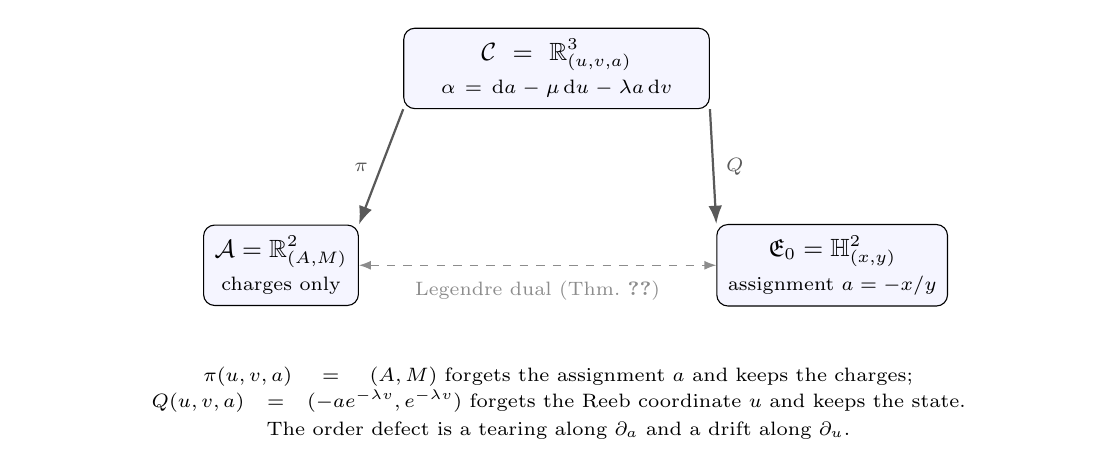
\begin{tikzpicture}[x=1cm,y=1cm,>=Latex,every node/.style={font=\small}]
  \node[draw,rounded corners,fill=blue!4,inner sep=4pt,align=center,
        text width=3.6cm] (C) at (0,3.1)
    {$\Cont=\R^3_{(u,v,a)}$\\[1pt]
     \scriptsize$\alpha=\mathrm da-\mu\,\mathrm du-\lambda a\,\mathrm dv$};
  \node[draw,rounded corners,fill=blue!4,inner sep=4pt,align=center] (A) at (-3.5,0.6)
    {$\ACS=\R^2_{(A,M)}$\\[1pt]\scriptsize charges only};
  \node[draw,rounded corners,fill=blue!4,inner sep=4pt,align=center] (H) at (3.5,0.6)
    {$\E_0=\HH^2_{(x,y)}$\\[1pt]\scriptsize assignment $a=-x/y$};
  \draw[->,thick,black!65] (C.south west) -- node[left=1pt,font=\scriptsize]
        {$\pi$} (A.north east);
  \draw[->,thick,black!65] (C.south east) -- node[right=1pt,font=\scriptsize]
        {$Q$} (H.north west);
  \draw[{Latex[length=1.5mm]}-{Latex[length=1.5mm]},dashed,black!45]
        (A.east) -- node[below=2pt,font=\scriptsize]
        {Legendre dual (Thm.~\ref{thm:dual-tearing})} (H.west);
  \node[font=\scriptsize,align=center,text width=13.2cm] at (0,-1.15)
    {$\pi(u,v,a)=(A,M)$ forgets the assignment $a$ and keeps the charges;\quad
     $Q(u,v,a)=(-ae^{-\lambda v},e^{-\lambda v})$ forgets the Reeb coordinate $u$
     and keeps the state.\\[2pt]
     The order defect is a tearing along $\pt_a$ and a drift along $\pt_u$.};
\end{tikzpicture}
\caption[The two projections of the contact model]%
{The two projections of the contact model, and their Legendre conjugacy.  The
charge projection $\pi$ forgets the assignment, so the order defect appears on
its fiber $\pt_a$ as a value tearing; the Reeb quotient $Q$ forgets the additive
charge, so the same defect appears on its fiber $\pt_u$ as a Reeb drift.
Section~\ref{sec:legendre} is the statement that these are two readings of one
contact curvature.}
\label{fig:two-projections}
\end{figure}

\subsection{The \AEG{} statements used, by compiled number}

All citations below are to the compiled numbering of the \AEG{} manuscripts
\cite{AEG0,AEG4}.  The working dialogue from which this note is drawn cited
several of them loosely; where the loose citation named a different statement
than the one actually used, the corrected reference is given here and the fact
is recorded in Appendix~\ref{app:register}.

{\small
\renewcommand{\arraystretch}{1.22}
\begin{longtable}{@{}p{0.215\linewidth}p{0.735\linewidth}@{}}
\toprule
reference & statement used here \\
\midrule
\endfirsthead
\toprule
reference & statement used here \\
\midrule
\endhead
\midrule
\multicolumn{2}{r}{\emph{continued}}\\
\endfoot
\bottomrule
\endlastfoot
Paper~0, Prop.~3.6 & the grid motions act on the assignment by
$a\circ\mathsf X_s=a+s$, $a\circ\mathsf Y_k=ka$. \\
Paper~0, Subsec.~3.4 & the five-row table of motions, including the reflection
$(x,y)\mapsto(-x,y)$ with $a\mapsto-a$. \\
Paper~0, Thm.~3.9 & continuous arithmetic motion:
$\frac{\mathrm d}{\mathrm ds}(a\circ\gamma)=\mu\cos\theta+\lambda(a\circ\gamma)\sin\theta$. \\
Paper~0, Thm.~4.2, Subsec.~4.3 & ripple pencils and ripple histories; the
common tangency point may move with the prefix. \\
Paper~0, Prop.~5.4, Subsec.~5.5 & fixed points of $z\mapsto a+b/z$ solve
$z^2-az-b=0$; general M\"obius fixed points are eigenlines. \\
Paper~0, Props.~7.1, 7.4 & affine cocycle and the left/right Maurer--Cartan
translation forms. \\
Paper~0, Def.~8.1, Prop.~8.2 & the \ACS{} and its weighted evaluation
$\hat\xi=\int_C e^{-M}\mathrm dA$. \\
Paper~0, Thm.~8.6 & only the multiplicative charge descends; the kernel word
$h(p,q)=\cM_q\cA_p\cM_{-q}\cA_{-e^{-q}p}$ has charges
$\bigl(p(1-e^{-q}),0\bigr)$. \\
Paper~0, Thm.~8.9 & weighted torsion--Stokes:
$\tau(\gamma,\delta)=\iint_{\Sigma}e^{M_*-M}\mathrm dA\wedge\mathrm dM$. \\
Paper~0, Props.~9.1, 9.6, 9.8, Thm.~9.2 & the contact form, its curvature
$\mu\lambda$, the Reeb quotient, and $d\alpha=-\mu\lambda Q^*\mathrm d\vol$. \\
Paper~0, Thm.~9.9 & dual tearing and Reeb drift: $\Delta a$ at fixed charges
versus $\Delta A=-\mu\lambda\,\mathrm{Area}_g(\Omega)$ at fixed state. \\
Paper~0, App.~D.1--D.2, D.4 & the oriented rectangle with pulled-back form
$pq\,\mathrm ds\wedge\mathrm dt$; the closed loop
$\ell=(\cA_p,\cM_q,\cA_{-p},\cM_{-q})$ with $\tau=p(1-e^{-q})$; Darboux
coordinates and $R=-(1/\mu)\pt_u$. \\
Paper~IV, Def.~3.1, Thms.~3.2, 3.3, 3.5 & regular bivaluations
$\Biv_K^{\mathrm{reg}}=\PP^1\!\times\!\PP^1\setminus\Delta$; the
bivaluation--projector bijection $\Pi_{a,b}=\frac1{1+ab}v_a\otimes\varphi_b$;
$G/H\cong\Biv_K^{\mathrm{reg}}$; the frame torsor. \\
Paper~IV, Prop.~3.7, Ex.~3.8 & finite-field counts
$|\PGL_2(\F_q)|=q(q^2-1)$, $|\Biv|=q(q+1)$, $|H|=q-1$; for $q=7$:
$336$, $56$, $6$. \\
Paper~IV, Prop.~4.9 & edge labels given only by ratios of frame lifts telescope
along every closed path. \\
Paper~IV, Def.~4.10, Thm.~4.11, Rem.~4.12, Ex.~4.13 & the incidence-coupled
transport $\mathcal T(\tilde e)\in\Aff(1,K)$, its Borel reduction, the
cross-ratio holonomy, the infinitesimal reductive connection, and the
$\F_7$ witness $\Lambda=4$. \\
Paper~IV, Prop.~10.1, Thm.~10.3 & Horner histories
$\xi=\sum_i d_i k^{n-i}$ and their histogram counts. \\
\end{longtable}}

\subsection{Notation and sign conventions}

The note keeps the \AEG{} conventions unchanged; a reader coming from the
manuscripts needs only the following table.

{\small
\renewcommand{\arraystretch}{1.2}%
\begin{longtable}{@{}ll@{}}
\toprule
symbol & meaning \\
\midrule
\endfirsthead
\toprule
symbol & meaning \\
\midrule
\endhead
\midrule
\multicolumn{2}{r}{\emph{continued}}\\
\endfoot
\bottomrule
\endlastfoot
$\E_0=(\HH^2,g_{\mu,\lambda},a)$ & basic hyperbolic arithmetic expression space;
$a(x,y)=-x/y$ \\
$u,v$ & arithmetic direction coordinates; $A=\mu u$, $M=\lambda v$ natural
charge coordinates \\
$a$ & assignment (the ``current arithmetic value''); on $\HH^2$, $a=-x/y$ \\
$\ACS=\R^2_{(A,M)}$ & accumulative commutative space; oriented by
$\mathrm dA\wedge\mathrm dM$ \\
$\Cont=\R^3_{(u,v,a)}$ & contact model; $\alpha=\mathrm da-\mathrm dA-a\,
\mathrm dM$ in charge coordinates \\
$\pi,\;Q$ & charge projection $\pi(u,v,a)=(A,M)$; Reeb quotient
$Q(u,v,a)=(-ae^{-\lambda v},e^{-\lambda v})$ \\
$q,\;p$ & ideal boundary point (asymptote) and ordinary point (finite scale) \\
$\cA_p,\;\cM_q$ & the additive and multiplicative motions, i.e. translation by
$p$ and dilation by $e^{q}$ \\
$h(p,q)$ & the kernel word of Thm.~8.6 \\
$\Pi_{a,b}$ & rank-one idempotent of the bivaluation $(a,b)$ \\
$q^+,q^-$ & image and kernel directions of a bivaluation (Paper~IV) \\
$B_\infty$ & $\Stab_{\PGL_2}(\infty)$, the affine Borel sector \\
$J$ & the inverting element $z\mapsto -1/z$ \\
$\Lambda(\square)$ & multiplicative cross-ratio holonomy of a four-step
bivaluation loop \\
$\mathcal T(e)$ & projective torsion transport of an edge \\
$\ell_0$ & short-distance reference length (ultraviolet cutoff) \\
$\mu,\;\lambda$ & arithmetic step constants; $\mu\lambda$ is the contact
curvature scalar \\
$\kappa$ & interaction curvature coefficient, $\kappa=q_1q_2$ by
Hypothesis~\ref{hyp:pairing} \\
\end{longtable}}

Two conventions matter and are used without further comment.  A history is
written chronologically from left to right, as in Paper~0: the word
$(\cM_q,\cA_p)$ first scales by $e^{q}$ and then translates by $p$.  Charges
are additive as a function on the history group: the total charge of a word is
the sum of its additive and multiplicative increments
(Convention~8.3 of Paper~0).  Composite maps act on the assignment by
composition in the reverse reading, so $(M_k\circ A_h)(a)=e^{q}(a+p)$ while
$(A_h\circ M_k)(a)=e^{q}a+p$; their difference is the elementary order defect
$p(e^{q}-1)$ of Appendix~D.3 of Paper~0.

\subsection{The five dictionary hypotheses}

Everything below is proved either from the \AEG{} statements of
Subsection~1.2 or from elementary computation, except at five points.  Each of
those is declared once here, is used in the sections named, and is not silently
converted into a theorem.

\begin{hypothesis}[Charge--motion dictionary]
\label{hyp:charge}
A charged particle at rest is an ideal-point-to-point history whose additive
steps carry the signed charge: the electron is generated by
$\cA_{-e}$, and the positron by $\cA_{+e}$, which by the reflection of
Paper~0, Subsection~3.4 satisfies $\mathcal R\circ\cA_{-e}\circ\mathcal R^{-1}
=\cA_{+e}$ with $\mathcal R(x,y)=(-x,y)$ scaling $a\mapsto-a$.  A virtual
photon exchange is one additive step of one history absorbed by another.
\end{hypothesis}

\begin{hypothesis}[Depth--distance dictionary]
\label{hyp:depth}
The multiplicative depth $e^{-M}$ of a history is the Coulomb kernel up to the
ultraviolet reference length,
\[
  e^{-M_*}=\frac{\ell_0}{r}
  \qquad\Longleftrightarrow\qquad
  M_*=\log\frac{r}{\ell_0},
\]
so that a scale interval $[0,M_*]$ represents a spatial separation $r$ and the
ultraviolet end $M=0$ represents the coincident limit.
\end{hypothesis}

\begin{hypothesis}[Curvature--energy dictionary]
\label{hyp:pairing}
The two-body interaction energy is the bilinear pairing of the two charges
against the contact curvature.  Concretely, writing the additive generator
strength $\mu\propto q_1$ and the multiplicative coupling $\lambda\propto q_2$,
the curvature scalar of Paper~0, Theorem~9.2 becomes
$\omega(D_u,D_v)=\mu\lambda\propto q_1q_2$, and the potential is the integral of
that density over the scale interval selected by Hypothesis~\ref{hyp:depth},
normalised by the three-dimensional solid angle $4\pi$.
\end{hypothesis}

\begin{hypothesis}[Velocity--tilt dictionary]
\label{hyp:velocity}
A charge moving with speed $v_{\mathrm{vel}}$ is a history whose depth coordinate
advances at rate $\beta=\mathrm dM/\mathrm d\tau=v_{\mathrm{vel}}/c$, i.e. the
direction angle of \eqref{eq:theta-flow} is the rapidity
$\theta=\operatorname{artanh}(v_{\mathrm{vel}}/c)$ of the motion, with $c$ the
critical rate at which the tilt saturates.
\end{hypothesis}

\begin{hypothesis}[Holonomy--radiation dictionary]
\label{hyp:radiation}
A nonvanishing projective holonomy of a closed history loop, in the sense of the
multiplicative component of Paper~IV, Theorem~4.11, is the carrier of
electromagnetic radiation: uniform motion has trivial holonomy and radiates
nothing, and an acceleration that moves the kernel coordinate produces a
holonomy whose magnitude measures radiated power.
\end{hypothesis}

\begin{statusbox}
\textbf{On the status of the hypotheses.}  None of the five is a theorem of
\AEG{}, and none is claimed to be.  Each is a dictionary: it names a physical
quantity by an \AEG{} object.  Hypotheses~\ref{hyp:charge} and
\ref{hyp:depth} fix what the ends and the scale variable of a history mean;
Hypothesis~\ref{hyp:pairing} fixes what an invariant of two histories means;
Hypothesis~\ref{hyp:velocity} fixes what motion means;
Hypothesis~\ref{hyp:radiation} fixes what a holonomy means.  The mathematical
content of every section stands without them; the physical conclusions are
conditional on them, and are stated in that form.  Section~\ref{sec:summary}
collects which conclusion rests on which hypothesis.

One further identification is made later and is not counted among the five
because it is a substitution rather than a dictionary: in
Section~\ref{sec:bohr} the assignment slot of the contact form is filled by the
scale-corrected radial momentum $r\,p_r$ (Lemma~\ref{lem:action-slot}).  It is
flagged there.
\end{statusbox}

\subsection{Roadmap}

{\small
\renewcommand{\arraystretch}{1.22}%
\begin{longtable}{@{}p{0.30\linewidth}p{0.16\linewidth}p{0.46\linewidth}@{}}
\toprule
source note & section & what it contributes \\
\midrule
\endfirsthead
\toprule
source note & section & what it contributes \\
\midrule
\endhead
\midrule
\multicolumn{3}{r}{\emph{continued}}\\
\endfoot
\bottomrule
\endlastfoot
\texttt{费曼图.md} & \S\ref{sec:feynman} & the $p_0\to p$ family as an operator
fiber; \ACS{} fan-out and bare-charge divergence; Reeb-fiber heights \\
\texttt{勒让德形式.md} & \S\ref{sec:legendre} & the exponential Legendre
identity and the dual tearing theorem \\
\texttt{电动力学讨论-01.md} & \S\ref{sec:coulomb} & Coulomb's sign rule from the
sign of $q_1q_2$; the dipole loop; the three geometric readings \\
\texttt{电动力学讨论-02.md} & \S\ref{sec:ampere}, \S\ref{sec:scattering} &
direction angle and the Amp\`ere coefficient; uniform motion in ripple
geometry; M\o ller versus Bhabha sectors \\
\texttt{电动力学讨论-02.md},
\texttt{电动力学讨论-03.md} & \S\ref{sec:radiation},
\S\ref{sec:torsion} & moving poles, cross-ratio holonomy, the torsion transport
and its Borel reduction \\
\texttt{电动力学讨论-03.md} & \S\ref{sec:bohr} & elliptic fixed points, Reeb
holonomy as action, Bohr--Sommerfeld quantization \\
--- & \S\ref{sec:summary} & dictionary table, status ledger, open ends \\
--- & App.~\ref{app:matrices}--\ref{app:register} & exact computations and the
register of verified identities \\
\end{longtable}}


\section{Ideal-Point Feynman Histories}
\label{sec:feynman}
% ---------------------------------------------------------------------
% Section 2
% ---------------------------------------------------------------------

\begin{cnread}
本节把「从理想点 $q$ 到普通点 $p$ 的一族穿线路径」严格写下来，并回答一个
具体问题：既然这些路径的起点终点都一样，它们在费曼图、\ACS{}、切触空间三个
视角下分别是什么？结论是：它们恰好是算子求值映射的一条纤维
$\rho^{-1}(g_{p_0\to p})$；在 \ACS{} 里摊成一条水平线段（裸荷随 $M\to\infty$
指数发散），在切触空间里则落在同一根 Reeb 纤维的\textbf{不同高度}上。
本节只用 Paper~0 的第 7--9 章，不需要任何物理字典。
\end{cnread}

\subsection{Two kinds of ideal point}

Let $\E_0=(\HH^2,g_{\mu,\lambda},a)$ be the basic model with
$a(x,y)=-x/y$.  In horocyclic coordinates $u=x$ and $y=e^{\lambda v}$ one has
$a=-ue^{-\lambda v}$, and the two affine motions of Paper~0,
Proposition~3.6, read
\begin{equation}\label{eq:grid-motions}
  \mathsf X_s(x,y)=(x-sy,\,y),
  \qquad
  \mathsf Y_k(x,y)=\Bigl(x,\frac yk\Bigr),
  \qquad
  a\circ\mathsf X_s=a+s,\quad a\circ\mathsf Y_k=ka .
\end{equation}
The ideal boundary $\pt_\infty\HH^2=\R\cup\{\infty\}$ carries two kinds of point,
and the distinction is used constantly below.

\begin{enumerate}[label=(\roman*)]
  \item The point at infinity, $q=i\infty$, i.e. $y\to+\infty$ or
  $M=\lambda v\to-\infty$.  This is the common base point of the
  Borel subgroup $B_\infty=\Stab_{\PGL_2}(\infty)$: every affine motion fixes
  it, so it is the natural origin of an affine history, and in the physical
  reading it is the ultraviolet, asymptotically free end.
  \item A finite ideal point $q=x_\infty\in\R$, i.e. $y\to0^{+}$ or
  $M\to+\infty$.  This is the infrared end, reached by unbounded positive
  scaling $\mathsf Y_{e^{M}}$ with $M\to+\infty$.
\end{enumerate}

\begin{remark}[Ultraviolet versus infrared end]
Whether one marches from $q=i\infty$ inward to $p$, or reads the same word
backwards from $p$ towards a finite ideal point, is a choice of direction, not a
choice of geometry: the two readings are the two ends of one word.  Paper~0
keeps both ends in view because the multiplicative charge is the only charge
that descends to the motion group (Theorem~8.6), so only $M$ can be compared
across histories without an order convention.
\end{remark}

\subsection{The family of histories is one operator fiber}

\begin{remark}[The ideal point is a direction, not a starting point]
\label{rem:q-is-a-direction}
$B_\infty$ fixes $q=i\infty$, so no affine motion carries $q$ to an interior
point of $\HH^2$: a history cannot literally start at the ideal point.  What the
phrase ``a history from $q$ to $p$'' means in this note, and what it means in
Paper~0's grid, is a history that starts at an ordinary point $p_0$ deep in the
ultraviolet region --- large $y_0$, near $q$ --- and ends at $p$.  The
formulation below therefore fixes $p_0$ explicitly.  Its distance from $q$ enters
only through the total multiplicative charge, and every invariant used in this
note is a function of the charges, not of how deep the start was placed.
\end{remark}

Fix an ordinary starting point $p_0=(x_0,y_0)\in\HH^2$ and an ordinary terminal
point $p=(x_p,y_p)\in\HH^2$.  A \emph{comb history} from $p_0$ to $p$ is a finite
chronological word
\begin{equation}\label{eq:comb-history}
  \gamma=(\cM_{m_1},\cA_{t_1},\cM_{m_2},\cA_{t_2},\dots,\cM_{m_n},\cA_{t_n}),
  \qquad m_i,t_i\in\R ,
\end{equation}
read from left to right, whose composite motion carries $p_0$ to $p$.  Here
$\cM_{m}$ denotes scaling by $e^{m}$ and $\cA_t$ translation by $t$; the word is
the left-expanded comb of Paper~0, Subsection~2.1.  In the comb notation of this
section we set the multiplicative step constant to $\lambda=1$, so that the
log-scale parameter $v$ and the multiplicative charge $M=\lambda v$ coincide;
the general case is recovered by the substitution $M=\lambda v$, and every
formula below is homogeneous in the charges.

\begin{proposition}[The $p_0\to p$ family is one operator fiber]
\label{prop:operator-fiber}
Let $g_{p_0\to p}\in B_\infty$ be the affine motion carrying $p_0$ to $p$.  Then
$\gamma$ in \eqref{eq:comb-history} carries $p_0$ to $p$ if and only if its
composite is $g_{p_0\to p}$.  Consequently the histories joining $p_0$ to $p$
are exactly one fiber of the evaluation map
$\rho:\Hist\to\Aff^{+}(1,\R)$ of Paper~0, Section~7.
\end{proposition}

\begin{proof}
$B_\infty$ acts simply transitively on $\HH^2$: it acts transitively because
$\mathsf Y_k$ and $\mathsf X_s$ of \eqref{eq:grid-motions} already carry any
point to any other, and freely because a nonidentity affine map has at most one
fixed point in $\HH^2$ (Paper~0, Proposition~5.4 with $b=0$; the pure
translation has none).  Hence exactly one affine motion carries $p_0$ to $p$,
and a word realizes that motion exactly when it equals $g_{p_0\to p}$ in the
group.
\end{proof}

Writing $g_{p_0\to p}(z)=e^{M_*}z+\xi_*$, the two invariants of the fiber are the
total multiplicative charge $M_*=\lambda\sum_i m_i$ and the total target
translation $\xi_*$.  In terms of the assignment,
\begin{equation}\label{eq:fiber-invariants}
  e^{M_*} = \frac{y_p}{y_0},
  \qquad
  a(p)=e^{M_*}a(p_0)+\xi_* = -\frac{x_p}{y_p}.
\end{equation}

\subsection{Comb diagrams and charge accounting}

The affine cocycle of Paper~0, Proposition~7.1, expresses the terminal
translation of a comb in two equivalent ways,
\begin{equation}\label{eq:comb-cocycle}
  \xi_\gamma=\sum_{i=1}^{n}t_i\,e^{\,M_{i+1:n}}
  = e^{M_*}\sum_{i=1}^{n}t_i\,e^{-M_i},
  \qquad M_{i:n}=\sum_{j=i}^{n}\lambda m_j .
\end{equation}
Read as a diagram, \eqref{eq:comb-cocycle} is a time-ordered Feynman diagram
with a single fermion line.

\begin{enumerate}[label=(\alph*)]
  \item The vertical segments $\cM_{m_i}$ are free propagation between
  vertices: they advance the scale by $e^{m_i}$ and cost no additive charge.
  \item The horizontal segments $\cA_{t_i}$ are vertex insertions at the scale
  shell $M_i$: each emits or absorbs one quantum and adds $t_i$ to the running
  value.
  \item The second form of \eqref{eq:comb-cocycle} says that a bare vertex
  inserted at depth $M_i$ contributes $t_ie^{-M_i}$ to the source-normalized
  charge and is then transported to the target frame by $e^{M_*}$.
\end{enumerate}

\begin{proposition}[The distributive law is the renormalisation resummation]
\label{prop:distributive-resummation}
Fix two vertices at distinct depths.  Then for every $M_1<M_*$ and $t_1$,
\[
  (\cM_{M_*-M_1},\cA_{t_1})\quad\text{and}\quad
  (\cA_{t_1e^{M_*-M_1}},\cM_{M_*-M_1})
\]
are histories with the same terminal operator but different total charges.  The
difference of their additive charges is the elementary order defect
$t_1\,(e^{M_*-M_1}-1)$.
\end{proposition}

\begin{proof}
Both words evaluate to the affine map $z\mapsto e^{M_*}z+e^{M_*-M_1}t_1$, which
is the content of the pointwise identity $k(z+p)=kz+kp$ of Paper~0,
Subsection~2.3.  Their additive charges are $t_1$ and $t_1e^{M_*-M_1}$, whose
difference is as displayed; the multiplicative charges agree.
\end{proof}

The proposition is the algebraic form of the statement that a large bare vertex
inserted deep in the ultraviolet can be transported to the infrared as a small
effective vertex.  In field-theoretic language the two words are the same
renormalized amplitude with the counterterm absorbed, and the charge difference
is the order defect that the \ACS{} will record as an area.

\subsection{The image in the accumulative commutative space}

Commutativizing forgets the order of the steps and keeps the two total charges
(Paper~0, Definition~8.1 and Proposition~8.5).  For the $p_0\to p$ family this has
an immediate consequence.

\begin{proposition}[The family fans out into a horizontal segment]
\label{prop:acs-fanout}
Let $\{\gamma\}$ be the histories of Proposition~\ref{prop:operator-fiber}.
Their \ACS{} charge chains $C_\gamma$ all terminate on the horizontal line
$M=M_*$, where $M_*$ is fixed by \eqref{eq:fiber-invariants}, and they satisfy
the single scalar constraint
\begin{equation}\label{eq:fanout-constraint}
  \hat\xi(p):=\int_{C_\gamma}e^{-M}\mathrm dA
  =\xi_*\,e^{-M_*}+a(q)
\end{equation}
of Paper~0, Proposition~8.2.  Along that line the total additive charge
$A_\gamma$ is not determined by $p$: a history that inserts its vertices early
needs $A_\gamma\to$ small, and one that inserts them late needs
$A_\gamma\asymp e^{M_*}\hat\xi(p)$.
\end{proposition}

\begin{proof}
The multiplicative charge is determined by the endpoint by
Theorem~8.6(3).  Proposition~8.2 identifies the weighted integral with the
source-normalized terminal translation, which is fixed by \eqref{eq:fiber-invariants}
because both ends are.  The two extremes are the two words of
Proposition~\ref{prop:distributive-resummation}: inserting at $M=0$ costs
$A=t_1$ and inserting at $M=M_*$ costs $A=t_1e^{M_*}$.
\end{proof}

\begin{corollary}[Two readings of the same divergence]
\label{cor:bare-divergence}
The quantity $A_\gamma$ --- the total additive charge, which the \ACS{} keeps as
its abscissa --- is not a function of the physical endpoint, and it grows like
$e^{M_*}$ for histories whose insertions are pushed to the infrared end.  The
weighted quantity $\hat\xi(p)$ is a function of the endpoint and stays finite.
\end{corollary}

\begin{warning}[What this does and does not explain]
\label{warn:divergence}
Corollary~\ref{cor:bare-divergence} says that the unweighted sum of insertions
over a scale range diverges like $e^{M}$ while its $e^{-M}$-weighted version does
not.  That is exactly the algebraic shape of the statement that a bare quantity
regularized at a short distance diverges while a renormalized quantity does not,
and the exponential weight is the usual scale factor.  It is \emph{not} a proof
of renormalizability of any field theory, and no loop integral is computed here.
The correspondence is between one exact \AEG{} identity and one structural
feature of the perturbative expansion.
\end{warning}

When two histories of the family also share their additive charge, they close up
in $\ACS$, and the weighted torsion--Stokes theorem of Paper~0, Theorem~8.9,
applies: the relative defect is
$\tau(\gamma,\delta)=\iint_{\Sigma_{\gamma\delta}}e^{M_*-M}\mathrm dA\wedge
\mathrm dM$.  For two such histories to \emph{also} reach the same $p$, that
torsion must vanish.  In the physical reading this is the statement that
cancellations between early and late insertions --- the finite remainders of
renormalization and the Ward-type identities --- are exactly the vanishing of a
signed weighted area.  The elementary case is the kernel word of
Theorem~8.6: the two histories $\gamma_1=(\cM_q,\cA_p)$ and
$\gamma_2=(\cA_{e^{-q}p},\cM_q)$ reach the same state and differ in additive
charge by $p(1-e^{-q})$, which is exactly the weighted area they enclose
(Lemma~\ref{lem:kernel-word}).

\subsection{The image in the contact model: Reeb heights}

Lift each history horizontally to $\Cont$: a curve $\tilde\gamma$ with
$\alpha(\dot{\tilde\gamma})=0$.  By Paper~0, Theorem~3.9 and the coordinate
form of the horizontal fields, this is the ordinary differential equation
$\mathrm da=\mu\,\mathrm du+\lambda a\,\mathrm dv$, and by
Proposition~9.8(2) its image under $Q$ is the arithmetic motion itself.

\begin{proposition}[Same state, different Reeb height]
\label{prop:reeb-heights}
Let $\tilde\gamma_1,\tilde\gamma_2$ be horizontal lifts of two histories of the
$p_0\to p$ family, starting at the same point of $\Cont$.  Then
$Q\circ\tilde\gamma_1$ and $Q\circ\tilde\gamma_2$ end at the same $p\in\HH^2$,
while
\[
  u(\tilde\gamma_1)-u(\tilde\gamma_2)=\frac{1}{\mu}\bigl(A_{\gamma_1}-A_{\gamma_2}\bigr).
\]
By Theorem~9.9 this height difference equals
$-\iint_{\Omega_{12}}\mathrm da\wedge\mathrm dM=-\mu\lambda\,\mathrm{Area}_g(\Omega_{12})$,
the hyperbolic area enclosed by the two projected paths in $\HH^2$.
\end{proposition}

\begin{proof}
Horizontal lifts of paths with the same endpoints in $\HH^2$ end on the same
fiber of $Q$ because $Q$ is the projection; the height difference is the
statement of Theorem~9.9(2), and the additive charge is $A=\mu u$ by the natural
charge coordinates of Appendix~D.4.
\end{proof}

\begin{figure}[t]
\centering
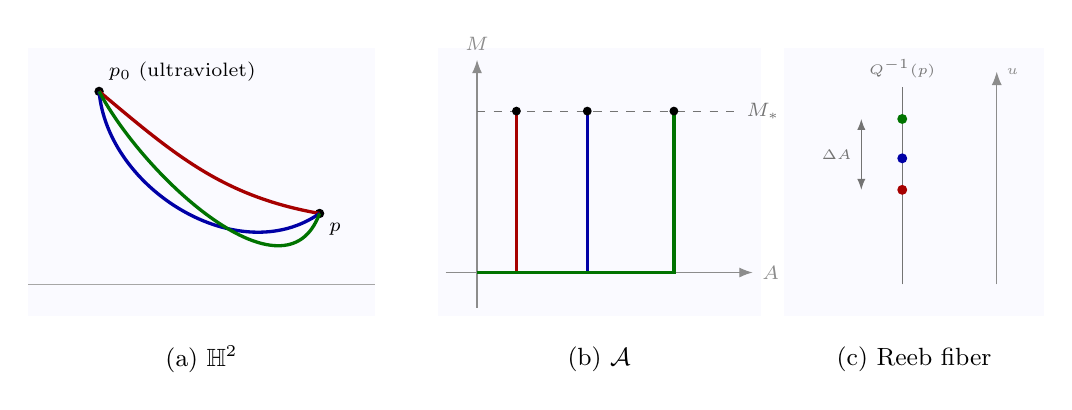
\begin{tikzpicture}[x=1cm,y=1cm,>=Latex,every node/.style={font=\scriptsize}]
  % ---- panel (a)
  \begin{scope}[shift={(0,0)}]
    \fill[blue!2] (-0.4,-0.4) rectangle (4.0,3.0);
    \draw[black!35] (-0.4,0)--(4.0,0);
    \fill (0.5,2.45) circle (1.7pt) node[above right] {$p_0$ (ultraviolet)};
    \fill (3.3,0.9) circle (1.7pt) node[below right] {$p$};
    \draw[very thick,red!65!black]   (0.5,2.45) to[out=-40,in=170] (3.3,0.9);
    \draw[very thick,blue!65!black]  (0.5,2.45) to[out=-85,in=215] (3.3,0.9);
    \draw[very thick,green!45!black] (0.5,2.45) to[out=-62,in=250] (3.3,0.9);
    \node[font=\small] at (1.8,-0.95) {(a) $\HH^2$};
  \end{scope}
  % ---- panel (b)
  \begin{scope}[shift={(5.3,0)}]
    \fill[blue!2] (-0.5,-0.4) rectangle (3.6,3.0);
    \draw[->,black!45] (-0.4,0.15)--(3.5,0.15) node[right] {$A$};
    \draw[->,black!45] (0,-0.3)--(0,2.85) node[above] {$M$};
    \draw[black!55,dashed] (0,2.2)--(3.3,2.2) node[right] {$M_*$};
    \draw[very thick,red!65!black]   (0,0.15)--(0.5,0.15)--(0.5,2.2);
    \draw[very thick,blue!65!black]  (0,0.15)--(1.4,0.15)--(1.4,2.2);
    \draw[very thick,green!45!black] (0,0.15)--(2.5,0.15)--(2.5,2.2);
    \fill (0.5,2.2) circle (1.6pt);
    \fill (1.4,2.2) circle (1.6pt);
    \fill (2.5,2.2) circle (1.6pt);
    \node[font=\small] at (1.55,-0.95) {(b) $\ACS$};
  \end{scope}
  % ---- panel (c)
  \begin{scope}[shift={(9.9,0)}]
    \fill[blue!2] (-0.7,-0.4) rectangle (2.6,3.0);
    \draw[black!55] (0.8,0.0)--(0.8,2.5) node[above,font=\tiny] {$Q^{-1}(p)$};
    \draw[->,black!45] (2.0,0.0)--(2.0,2.7) node[right,font=\tiny] {$u$};
    \fill[red!65!black]   (0.8,1.2) circle (1.8pt);
    \fill[blue!65!black]  (0.8,1.6) circle (1.8pt);
    \fill[green!45!black] (0.8,2.1) circle (1.8pt);
    \draw[{Latex[length=1.4mm]}-{Latex[length=1.4mm]},black!55]
      (0.28,1.2)--(0.28,2.1) node[midway,left,font=\tiny] {$\Delta A$};
    \node[font=\small] at (0.95,-0.95) {(c) Reeb fiber};
  \end{scope}
\end{tikzpicture}
\caption[Three images of one family of histories]%
{Three images of one family of histories.  (a) In $\HH^2$ the histories have the
same two endpoints and therefore the same composite operator.  (b) In $\ACS$ they
share the multiplicative charge $M_*$ and differ in additive charge $A_\gamma$,
subject to the weighted constraint \eqref{eq:fanout-constraint}.  (c) In $\Cont$
they terminate on one Reeb fiber over $p$ at distinct heights
$u_\gamma=A_\gamma/\mu$; the height spread equals the hyperbolic area enclosed by
the projected paths (Theorem~\ref{thm:dual-tearing}).}
\label{fig:fanout}
\end{figure}

\begin{remark}[Action and phase]
\label{rem:prequantum}
The Reeb coordinate $u$ is the coordinate along which the contact form evaluates
to $1$: $\alpha(R)=1$ with $R=-\tfrac1\mu\pt_u$ (Appendix~D.4 of Paper~0).  In
the geometric quantization of a contact manifold, the Reeb direction is the
circle fiber of the prequantum bundle and its coordinate is the phase of the
wave function \cite{Geiges2008,BoothbyWang1958}.  Proposition~\ref{prop:reeb-heights}
therefore says that histories reaching the same state with different Reeb
heights differ by a phase.  Summing over the fiber with weights
$e^{\,\mathrm i\,A_\gamma}$ is then the natural candidate for a path integral in
this picture.  Nothing in this note depends on that candidate, which is recorded
as a target rather than as a result.
\end{remark}

\subsection{Radix shells}

If the scaling steps are quantized on a $k$-ary grid and each shell either emits
or does not, the word becomes a Horner expansion and the terminal translation is
\begin{equation}\label{eq:horner}
  \xi=\sum_{i=1}^{n}d_i\,k^{\,n-i},
  \qquad d_i\in\{0,1,\dots,k-1\},
\end{equation}
with the counting statements of Paper~IV, Proposition~10.1 and Theorem~10.3.  In
the physical reading $d_i\ne0$ at shell $i$ records a virtual process at the
Wilsonian momentum shell $k^{n-i}$, and the terminal value is built up shell by
shell from the ultraviolet end.  Once signed and continuous increments are
allowed, the number of histories sharing one terminal operator is infinite,
which is the content of Proposition~\ref{prop:operator-fiber}.

\subsection{Panorama}

\begin{center}\small
\renewcommand{\arraystretch}{1.25}
\begin{tabular}{@{}p{0.19\linewidth}p{0.24\linewidth}p{0.24\linewidth}p{0.23\linewidth}@{}}
\toprule
carrier & \AEG{} object & Feynman reading & invariant that survives \\
\midrule
$\E_0$ & broken-line family from $q=\infty$ to $p$; one fiber
$\rho^{-1}(g_{p_0\to p})$
& time- and scale-ordered comb diagrams from the asymptotic state to the dressed
state
& endpoint assignment $a(p)$ and total scale $e^{M_*}$ fixed; the order of
insertions is retained \\
$\ACS$ & all chains end on $M=M_*$; abscissa $A_\gamma=\sum t_i$ free subject to
\eqref{eq:fanout-constraint}
& bare versus renormalized charge; ultraviolet sensitivity of the unweighted sum
& $\hat\xi(p)=\int_{C}e^{-M}\mathrm dA$; and
$\tau(\gamma,\delta)=0$ when both charge and endpoint agree \\
$\Cont$ & Legendrian lift family; endpoints on distinct heights of
$Q^{-1}(p)$
& different histories for one physical state, carrying different phases
& Reeb drift $A_{\gamma_1}-A_{\gamma_2}
=-\mu\lambda\,\mathrm{Area}_g(\Omega_{12})$ \\
\bottomrule
\end{tabular}
\end{center}

Section~\ref{sec:legendre} isolates the last row as a theorem about pairs of
histories and then re-reads the first row as its conjugate.


\section{The Legendre Form: Charge Projection versus Reeb Quotient}
\label{sec:legendre}
% ---------------------------------------------------------------------
% Section 3
% ---------------------------------------------------------------------

\begin{cnread}
本节回答一个自然的问题：切触空间里那两个投影 $\pi$（忘掉赋值 $a$）与
$Q$（忘掉 Reeb 荷 $u$）之间的「勒让德对偶」，究竟与力学里联系
Lagrange 量和 Hamilton 量的\textbf{勒让德变换}是不是同一件事？答案是：
在标准切触流形上，它就是同一个操作的两个 Legendre 叶层。
由此得到本文的第一个真正的新命题：\textbf{双重撕裂定理}——固定荷看
「赋值撕裂 $\Delta a$」（Paper~0 定理 8.9），固定状态看「Reeb 纤维漂移
$\Delta A$」（Paper~0 定理 9.9），两者是同一个切触曲率的两个共轭读法。
本节末尾用核字 $h(p,q)$ 做两条路径的现场验算，结果一字不差是
$p(1-e^{-q})$。
\end{cnread}

\subsection{Why the mechanical Legendre transform is a contact statement}

In analytical mechanics with one degree of freedom, let $q$ be the coordinate,
$p$ the momentum, and $S$ the action, so that $(q,p,S)$ are coordinates on the
first jet bundle $J^1(\R)\cong\R^3$.  The canonical contact form is
\begin{equation}\label{eq:mech-contact}
  \alpha_{\mathrm{mech}}=\mathrm dS-p\,\mathrm dq=0 .
\end{equation}
Using $\mathrm d(pq)=p\,\mathrm dq+q\,\mathrm dp$ and putting
$\tilde S:=pq-S$, the same form reads
\begin{equation}\label{eq:mech-contact-dual}
  \alpha_{\mathrm{mech}}=-\mathrm d\tilde S+q\,\mathrm dp=0 .
\end{equation}
Equations \eqref{eq:mech-contact} and \eqref{eq:mech-contact-dual} are the same
one-form written through two different choices of potential, and the two
choices are related by the Legendre transformation.  Geometrically the content
is that one contact three-manifold carries two Legendrian fibrations: the
``coordinate'' projection $(q,p,S)\mapsto(q,S)$ in which $p\,\mathrm dq$ is read
as the accumulated quantity, and the ``momentum'' projection in which
$q\,\mathrm dp$ is.  Nothing about the contact structure changes; what changes is
which variable is declared to be a function of the others.

\begin{remark}[What the Legendre transformation does not do]
The passage from \eqref{eq:mech-contact} to \eqref{eq:mech-contact-dual} uses
only the product rule.  It is therefore available wherever the product exists;
the analytic content of the classical Legendre transformation (convexity,
invertibility of $p=\partial S/\partial q$) is not used and is not needed here.
\end{remark}

\subsection{The arithmetic contact form and its two potentials}

In the natural charge coordinates $A=\mu u$ and $M=\lambda v$ of Paper~0,
Appendix~D.4, the arithmetic contact form is
\begin{equation}\label{eq:arith-contact}
  \alpha=\mathrm da-\mathrm dA-a\,\mathrm dM,
\end{equation}
and the global affine change of coordinates
\begin{equation}\label{eq:darboux}
  x_{\mathrm D}=M,
  \qquad
  y_{\mathrm D}=a,
  \qquad
  z_{\mathrm D}=a-A
\end{equation}
puts it in standard Darboux form $\alpha=\mathrm dz_{\mathrm D}-y_{\mathrm D}
\,\mathrm dx_{\mathrm D}$ (Appendix~D.4).  Comparing \eqref{eq:darboux} with
\eqref{eq:mech-contact} identifies the correspondence
\begin{equation}\label{eq:legendre-dictionary}
  S\;\longleftrightarrow\; a-A,
  \qquad
  p\;\longleftrightarrow\;a,
  \qquad
  q\;\longleftrightarrow\;M .
\end{equation}
The current assignment $a$ plays the role of the momentum, and the logarithmic
scale $M$ plays the role of the coordinate.

\begin{lemma}[Legendre-dual form of $\alpha$]
\label{lem:legendre-linear}
With $\tilde S:=aM-a+A$ one has the identity
\begin{equation}\label{eq:legendre-linear}
  \alpha=-\mathrm d\tilde S+M\,\mathrm da
  \qquad\text{on }\Cont .
\end{equation}
\end{lemma}

\begin{proof}
Expanding $-\mathrm d(aM-a+A)+M\,\mathrm da$ gives
$-(a\,\mathrm dM+M\,\mathrm da-\mathrm da+\mathrm dA)+M\,\mathrm da
=\mathrm da-\mathrm dA-a\,\mathrm dM$.
\end{proof}

\begin{remark}[A correction to the working note]
\label{rem:legendre-correction}
The working note from which this section is drawn displayed the same step with
the coefficient $1+M$ on $\mathrm da$, that is
$\alpha=-\mathrm d(A+aM-a)+(1+M)\mathrm da$.  Expanding shows that this has an
extra $\mathrm da$ and is not $\alpha$.  The correct dual potential is
$A+aM-a$ with momentum coefficient $M$, as in \eqref{eq:legendre-linear}.  The
error does not propagate: every later identity in the note uses the
exponential form \eqref{eq:legendre-exponential} below, which is correct as
written.  Check~V5.1--V5.2 of Appendix~\ref{app:register} records both.
\end{remark}

The linear Legendre transformation \eqref{eq:legendre-linear} is not the most
intrinsic one available here, because the multiplicative motion of \AEG{} is the
exponential $e^{M}$ rather than the addition of $M$.  Rescaling the contact
form by the nowhere-vanishing factor $e^{-M}$ --- which leaves the horizontal
distribution $\ker\alpha$ untouched --- gives a second, multiplicative dual.

\begin{lemma}[Exponential Legendre identity]
\label{lem:legendre-exponential}
On $\Cont$,
\begin{equation}\label{eq:legendre-exponential}
  e^{-M}\alpha=\mathrm d\bigl(e^{-M}a\bigr)-e^{-M}\mathrm dA .
\end{equation}
\end{lemma}

\begin{proof}
$e^{-M}\alpha=e^{-M}(\mathrm da-a\,\mathrm dM)-e^{-M}\mathrm dA$ and
$\mathrm d(e^{-M}a)=e^{-M}\mathrm da-a e^{-M}\mathrm dM$.
\end{proof}

\begin{remark}[Three names for one quantity]
\label{rem:hat-a}
The quantity $\hat a:=e^{-M}a$ occurring in \eqref{eq:legendre-exponential} has
three readings.  It is the source-normalized assignment of Paper~0,
Proposition~8.2; it is minus the horizontal coordinate of the basic hyperbolic
model, because under the Reeb quotient
$Q(u,v,a)=(-ae^{-\lambda v},e^{-\lambda v})$ one has $\hat a=-x$; and it is, by
Lemma~\ref{lem:legendre-exponential}, the potential whose differential measures
the additive charge in the target frame.  Paper~0, Theorem~9.9 is exactly the
statement that these three readings agree.
\end{remark}

\subsection{The dual tearing theorem}

The two readings of Lemmas~\ref{lem:legendre-linear}
and~\ref{lem:legendre-exponential} become two comparison experiments.  The
statement below is Paper~0, Theorem~9.9; it is reproduced here in the notation
of this note because every later section uses it.

\begin{theorem}[Dual tearing and Reeb drift]
\label{thm:dual-tearing}
Let $\tilde\gamma_1,\tilde\gamma_2$ be piecewise smooth horizontal lifts in
$\Cont$ with a common initial state.
\begin{enumerate}[label=(\arabic*)]
  \item \emph{(Fixed charges: value tearing.)}  Suppose the projected charge
  chains $C_i=\pi\circ\tilde\gamma_i$ share their terminal point $(A_*,M_*)$.
  Then the terminal assignments differ by
  \begin{equation}\label{eq:value-tearing}
    a(\tilde\gamma_1(1))-a(\tilde\gamma_2(1))
    =e^{M_*}\oint_{C_1-C_2}e^{-M}\mathrm dA
    =\iint_{\Sigma_{12}}e^{M_*-M}\mathrm dA\wedge\mathrm dM
    =\tau(\gamma_1,\gamma_2),
  \end{equation}
  for any oriented two-chain $\Sigma_{12}$ in $\ACS$ with
  $\pt\Sigma_{12}=C_1-C_2$.  This is the weighted torsion--Stokes formula of
  Paper~0, Theorem~8.9.
  \item \emph{(Fixed state: Reeb drift.)}  Suppose instead that the projected
  paths $\tilde\gamma_i=Q\circ\tilde\gamma_i$ terminate at the same point
  $p\in\HH^2$, equivalently at the same pair $(M_*,a_*)$.  Then the terminals
  lie on the same Reeb fiber and
  \begin{equation}\label{eq:reeb-drift}
    \Delta A:=A(\tilde\gamma_1(1))-A(\tilde\gamma_2(1))
    =-\oint_{\tilde\gamma_1-\tilde\gamma_2}a\,\mathrm dM
    =-\iint_{\Omega_{12}}\mathrm da\wedge\mathrm dM
    =-\mu\lambda\,\mathrm{Area}_{g_{\mu,\lambda}}(\Omega_{12}),
  \end{equation}
  for any oriented two-chain $\Omega_{12}\subset\HH^2$ with
  $\pt\Omega_{12}=\tilde\gamma_1-\tilde\gamma_2$.
\end{enumerate}
\end{theorem}

\begin{proof}
(1) Integrate \eqref{eq:legendre-exponential} along each horizontal lift; the
initial terms cancel on subtraction, and $e^{M_*}$ multiplying the result gives
the first equality.  The second is Stokes' theorem in $\ACS$ with the target
weight $e^{M_*-M}$, as in Paper~0, Theorem~8.9.

(2) Integrate \eqref{eq:arith-contact} along each lift to get
$A(\tilde\gamma_i(1))-A_0=(a(\tilde\gamma_i(1))-a_0)-\int_{\tilde\gamma_i}
a\,\mathrm dM$.  Under common terminal state the boundary terms cancel on
subtraction, giving the line-integral form.  Stokes' theorem in $\HH^2$ and
$d\alpha=-\mu\lambda\,Q^*\mathrm d\vol_{g_{\mu,\lambda}}$ of Paper~0,
Proposition~9.8(5) give the area form.
\end{proof}

\begin{remark}[Why the two projections must be conjugate]
\label{rem:conjugacy}
$\pi$ forgets the assignment fiber $\pt_a$ and $Q$ forgets the Reeb fiber
$\pt_u$.  These are different directions of one three-manifold, so a comparison
that closes in one projection necessarily fails to close in the other: a
charge-compatible pair stays open on $\HH^2$, and a state-compatible pair closes
on $\HH^2$ and opens along the Reeb fiber.  That complementarity --- not an
analogy --- is the content of the word ``duality'' here.
\end{remark}

\subsection{A worked pair: the kernel word}

The smallest nontrivial instance is the element of $\ker\nu$ exhibited in
Paper~0, Theorem~8.6,
\begin{equation}\label{eq:kernel-word}
  h(p,q)=\cM_q\,\cA_p\,\cM_{-q}\,\cA_{-e^{-q}p},
\end{equation}
whose two halves are the prefixes $\gamma_1=(\cM_q,\cA_p)$ and
$\gamma_2=(\cA_{e^{-q}p},\cM_q)$.  Both carry $(M,a)=(0,0)$ to the same terminal
state with $M_*=q$ and $a_*=p$.

\begin{lemma}[Reeb drift of the kernel word]
\label{lem:kernel-word}
For $\gamma_1,\gamma_2$ as above,
\[
  \Delta A=A(\gamma_1)-A(\gamma_2)=p-e^{-q}p=p(1-e^{-q}),
\]
and the two sides of \eqref{eq:reeb-drift} both evaluate to $p(1-e^{-q})$.  The
weighted torsion of \eqref{eq:value-tearing} for the same pair vanishes, as it
must, since the terminal assignments agree.
\end{lemma}

\begin{proof}
The bare additive charges are $A(\gamma_1)=p$ and $A(\gamma_2)=e^{-q}p$.  On the
state side, $\gamma_1$ is the lower broken line $(0,0)\to(q,0)\to(q,p)$ with
$a\equiv0$ along its horizontal leg, so $\int_{\gamma_1}a\,\mathrm dM=0$, while
$\gamma_2$ follows $a(M)=pe^{M-q}$ and
$\int_{\gamma_2}a\,\mathrm dM=\int_0^q pe^{M-q}\mathrm dM=p(1-e^{-q})$.
Hence $-\bigl(\int_{\gamma_1}-\int_{\gamma_2}\bigr)a\,\mathrm dM=p(1-e^{-q})$,
in agreement with the charge difference.  The weighted area route gives
$\int_0^q\!\!\int_0^p e^{-M}\mathrm dA\,\mathrm dM=p(1-e^{-q})$ as well.  The
verification is Check~V6.1--V6.3.
\end{proof}

This is the identity that Paper~0, Appendix~D.2 records as the archetype of
``zero total charge is weaker than operator neutrality'': the loop
$\ell=(\cA_p,\cM_q,\cA_{-p},\cM_{-q})$ has total charge $(0,0)$ yet
$\tau(\ell,\varnothing)=p(1-e^{-q})$.  In Section~\ref{sec:coulomb} this lemma is
read as the binding energy of a charge dipole, and in
Section~\ref{sec:radiation} it is read as the phase carried by a virtual pair.

\subsection{The duality table}

\begin{center}\small
\renewcommand{\arraystretch}{1.3}
\begin{tabular}{@{}p{0.22\linewidth}p{0.36\linewidth}p{0.36\linewidth}@{}}
\toprule
 & \textbf{reading A: charge projection $\pi$} & \textbf{reading B: Reeb quotient
 $Q$} \\
\midrule
map & $\Cont\to\ACS_{(A,M)}$, forgets $a$
& $\Cont\to\E_0$, forgets $u=A/\mu$ \\
form used & $e^{-M}\alpha=\mathrm d(e^{-M}a)-e^{-M}\mathrm dA$
& $\alpha=-\mathrm dA+(\mathrm da-a\,\mathrm dM)$ \\
closure hypothesis & same terminal charges $(A_*,M_*)$
& same terminal state $p=(M_*,a_*)$ \\
vertical defect & value tearing $\Delta a$
& Reeb drift $\Delta A=\mu\Delta u$ \\
value & $\Delta a=\iint_\Sigma e^{M_*-M}\mathrm dA\wedge\mathrm dM$
& $\Delta A=-\iint_\Omega\mathrm da\wedge\mathrm dM
=-\mu\lambda\,\mathrm{Area}_g(\Omega)$ \\
\AEG{} source & Theorem~8.9, Prop.~8.2
& Theorem~8.6, Prop.~9.8, Theorem~9.9 \\
\bottomrule
\end{tabular}
\end{center}

\subsection{The open thread: from the affine sector to the projective group}

Both readings above live in the affine sector: the horizontal lifts are lifts
inside $B_\infty$, and the Riccati structure of the assignment along a flow is
hidden.  If one allows the second-slot division $c/z$, i.e. the inverting
element $J(z)=-1/z$, then the same one-form acquires a quadratic term and the
assignment obeys a Riccati rather than a linear equation.  Section~\ref{sec:radiation}
carries out exactly that step, and shows that the additional datum which then
appears --- the kernel coordinate $b$ of the bivaluation --- is what makes a
closed history carry a non-telescoping holonomy.


\section{Electrostatics: Coulomb's Law from Contact Curvature}
\label{sec:coulomb}
% ---------------------------------------------------------------------
% Section 4
% ---------------------------------------------------------------------

\begin{cnread}
本节是全文的第一次「校准」：把第 3 节的双重撕裂定理用到两个静止电荷上，
看能不能不借助任何外加的闵氏度规，直接从 \AEG{} 的几何量里读出库仑定律的
\textbf{符号规律}（同号相斥、异号相吸）。做法是：把两个电荷写成两次加法步
$q_1,q_2$，相互作用能取为切触曲率的双线性配对 $\omega(D_u,D_v)=\mu\lambda$，
于是 $\kappa=q_1q_2$ 的符号就是势能的符号；而正电子的 $+e$ 由 Paper~0
第 3.4 小节的反射算子给出，它恰好翻转了 2-链的定向（附录 D.1）。
本节 4.6 小节逐条列出哪些是已证事实、哪些是字典假设。
\end{cnread}

\subsection{Stage and dictionary}

Work on $\E_0$ and its contact model with the natural charge coordinates
$(A,M)$ of \eqref{eq:arith-contact}.  Two charges at rest are two ideal-point
histories whose multiplicative charges are equal, because both sit at the same
spatial separation from the observation point in the
Hypothesis~\ref{hyp:depth} sense,
\begin{equation}\label{eq:depth-distance}
  e^{-M_*}=\frac{\ell_0}{r}
  \qquad\Longleftrightarrow\qquad
  M_*=\log\frac{r}{\ell_0},
\end{equation}
so that $M=0$ is the ultraviolet reference (coincident limit) and $M_*\to\infty$
is infinite separation.  Charge 1 injects its additive step at the ultraviolet
end; the field it creates at the location of charge 2 is the assignment reached
after the scale step $M_*$,
\begin{equation}\label{eq:field-at-2}
  a_1(p)=q_1\,e^{-M_*}=\frac{q_1\ell_0}{r},
\end{equation}
which under \eqref{eq:depth-distance} is the Coulomb kernel up to the reference
length.

The two signs of charge are the two signs of the additive generator.

\begin{lemma}[Reflection conjugates the electron step into the positron step]
\label{lem:reflection}
Let $\mathcal R(x,y)=(-x,y)$ be the reflection of Paper~0, Subsection~3.4, which
acts on the assignment by $a\mapsto-a$, and let $\mathsf X_s$ be the
translation \eqref{eq:grid-motions}.  Then
\[
  \mathcal R\circ\mathsf X_{-e}\circ\mathcal R^{-1}=\mathsf X_{+e},
  \qquad\text{equivalently}\qquad
  a\circ\mathcal R\circ\mathsf X_{-e}\circ\mathcal R^{-1}=a+e .
\]
\end{lemma}

\begin{proof}
$\mathcal R^{-1}=\mathcal R$, and for a point $(x,y)$,
$\mathcal R(x,y)=(-x,y)$, then
$\mathsf X_{-e}(-x,y)=(-x+ey,y)$, then $\mathcal R(-x+ey,y)=(x-ey,y)
=\mathsf X_{+e}(x,y)$.
\end{proof}

\begin{warning}[The reflection is not one of the four operations]
\label{warn:reflection}
Paper~0, Subsection~3.4 is explicit that the reflection is not itself one of the
four arithmetic operations: it appears because the assignment of the model is
signed, and it is the elementary instance of the second-slot subtraction $c-z$.
Multiplication by a negative constant is the reflection composed with a positive
scaling.  Lemma~\ref{lem:reflection} must be read with that restriction: what is
conjugated is the additive motion, and the conjugation uses a map that is
outside the positive affine group.
\end{warning}

\subsection{The exchange and the interaction energy}

Consider the two histories of the exchange: charge 1 emits at the ultraviolet
end and the field is transported to charge 2, and the conjugate history in which
charge 2 emits and the field is transported back.  They are the histories
$\gamma_1$ and $\gamma_2$ of Lemma~\ref{lem:kernel-word}, with additive steps
$q_1,q_2$ in place of $p$ and multiplicative charge $M_*$ in place of $q$.

The interaction energy is then obtained in either of two equivalent ways.

\begin{enumerate}[label=(\alph*)]
  \item \emph{Pairing of field and copoint.}  The displacement of the assignment
  produced by charge 1 at the location of charge 2 is
  $\Delta a_1(r)=q_1\ell_0/r$; contracting it with the dual functional carried by
  charge 2 gives, after the $4\pi$ solid-angle normalisation,
  \begin{equation}\label{eq:pairing-energy}
    V(r)=\frac{1}{4\pi\ell_0}\,q_2\,\Delta a_1(r)
       =\frac{q_1q_2}{4\pi r} .
  \end{equation}
  \item \emph{Contact curvature density.}  Do not pair externally.  Instead let
  the additive generator strength be $\mu\propto q_1$ and the multiplicative
  coupling be $\lambda\propto q_2$.  Then the curvature scalar of Paper~0,
  Theorem~9.2 is
  \begin{equation}\label{eq:kappa}
    \omega(D_u,D_v)=\mu\lambda\;\propto\;q_1q_2=:\kappa ,
  \end{equation}
  and integrating the density over the scale interval $[0,M_*]$ selected by
  \eqref{eq:depth-distance} gives the same
  $V(r)=\kappa\,e^{-M_*}/(4\pi\ell_0)=\kappa/(4\pi r)$.
\end{enumerate}

Reading (b) is the one that carries the sign for free: by Theorem~9.2 the
curvature scalar of the horizontal distribution is literally $\mu\lambda$, and by
Remark~9.5 of Paper~0 it is an intrinsic invariant of the distribution even
though its numerical value depends on the choice of horizontal metric.  The sign
of $\kappa$ is therefore the sign of the product of the two charge steps, and
that is the whole of the sign rule.

\begin{statusbox}
\textbf{Where Hypothesis~\ref{hyp:pairing} enters.}  Theorem~9.2 supplies
$\omega(D_u,D_v)=\mu\lambda$ as an exact statement about the contact
distribution.  It does not by itself say that $\lambda$ is proportional to a
second charge, nor that the integral of the density over a scale interval is an
energy.  Both are the content of Hypothesis~\ref{hyp:pairing}, and the force law
below is conditional on it.  What is \emph{not} hypothetical is the sign
structure: once $\kappa=q_1q_2$, the two cases differ by the sign of a product
of two real numbers, and no further choice is available.
\end{statusbox}

\subsection{Like charges: the two-electron case}

Take $q_1=q_2=-e$.  Then
\begin{equation}\label{eq:kappa-ee}
  \kappa_{ee}=q_1q_2=(-e)(-e)=+e^{2}>0,
\end{equation}
which is the same sign as for two positive charges.  Geometrically this is
Lemma~\ref{lem:reflection} applied twice: the two reflections of the second
slot compose to the identity, $\mathcal R^2=\id$, so the 2-chain keeps its
orientation.  Paper~0, Appendix~D.1 makes the same statement at the level of the
oriented rectangle: the pulled-back orientation form is $pq\,\mathrm ds\wedge
\mathrm dt$, so a double sign change leaves it $+pq\,\mathrm ds\wedge\mathrm dt$.

Integrating the curvature density over the scale interval as in
\eqref{eq:pairing-energy},
\begin{equation}\label{eq:V-ee}
  V_{ee}(r)=\frac{\kappa_{ee}}{4\pi\ell_0}e^{-M_*}=+\frac{e^{2}}{4\pi r}>0 .
\end{equation}
The generalized force conjugate to the separation $r$ is
\begin{equation}\label{eq:F-ee}
  F_{ee}(r)=-\frac{\mathrm dV_{ee}}{\mathrm dr}
  =-\frac{\mathrm d}{\mathrm dr}\Bigl(+\frac{e^{2}}{4\pi r}\Bigr)
  =+\frac{e^{2}}{4\pi r^{2}}>0,
\end{equation}
i.e. directed along increasing $r$: the charges are pushed apart.

\begin{remark}[Why a positive potential means repulsion here]
\label{rem:relaxation}
The sign convention is the one fixed in Section~1.3: $V$ is the energy of the
configuration as a function of the separation, so $F=-\mathrm dV/\mathrm dr$ is
the force conjugate to $r$.  In the $\E_0$ reading of
Subsection~\ref{subsec:three-readings} below, $V_{ee}>0$ is exactly the
statement that the configuration relaxes towards $r\to\infty$, i.e. towards
$e^{-M}\to0$ on the ideal boundary.
\end{remark}

\subsection{Opposite charges: the electron--positron case}

Take $q_1=-e$ and $q_2=+e$.  By Lemma~\ref{lem:reflection} the second charge is
the first one conjugated by the reflection, so exactly one side of the 2-chain
carries a sign change.

\begin{lemma}[Orientation reversal for exactly one negative side]
\label{lem:orientation}
For the oriented singular rectangle $R_{p,q}(s,t)=(sp,tq)$ with
$0\le s,t\le1$ of Paper~0, Appendix~D.1, the pulled-back orientation form is
$pq\,\mathrm ds\wedge\mathrm dt$.  Hence the orientation of the rectangle
reverses exactly when one of $p,q$ changes sign, and the weighted integral
$\int_{R_{p,q}}e^{q-M}\mathrm dA\wedge\mathrm dM=p(e^{q}-1)$ is unchanged.
\end{lemma}

\begin{proof}
$R_{p,q}^*(\mathrm dA\wedge\mathrm dM)=pq\,\mathrm ds\wedge\mathrm dt$; the
weight is positive, so the sign of the integral is the sign of $pq$.  The value
$p(e^q-1)$ follows by direct integration as in Appendix~D.1.
\end{proof}

Consequently the curvature pairing changes sign,
\begin{equation}\label{eq:kappa-ep}
  \kappa_{e^+e^-}=q_1q_2=(-e)(+e)=-e^{2}<0,
\end{equation}
and with it the potential and the force:
\begin{equation}\label{eq:V-ep}
  V_{e^+e^-}(r)=-\frac{e^{2}}{4\pi r}<0,
  \qquad
  F_{e^+e^-}(r)=-\frac{e^{2}}{4\pi r^{2}}<0 .
\end{equation}
The force is along decreasing $r$: the charges are pulled together.

Two further \AEG{} identities describe the same case.

\begin{proposition}[The neutral pair is the closed charge loop]
\label{prop:dipole-loop}
For equal and opposite additive steps the total additive charge vanishes,
$A_{\mathrm{tot}}=(-e)+(+e)=0$, and the pair is realized by the closed
chronological loop
$\ell=(\cA_{+e},\cM_{M_*},\cA_{-e},\cM_{-M_*})$ of Paper~0, Appendix~D.2.  Its
weights satisfy
\[
  \tau(\ell,\varnothing)=e\bigl(1-e^{-M_*}\bigr)=e\Bigl(1-\frac{\ell_0}{r}\Bigr),
\]
which vanishes as $r\to\ell_0$ and grows towards $e$ as $r\to\infty$.
\end{proposition}

\begin{proof}
The charge computation is Theorem~8.6(2) with $(p,q)\mapsto(e,M_*)$; the
evaluation defect is the lemma of Section~3.5.  The limits are immediate from
\eqref{eq:depth-distance}.
\end{proof}

\begin{remark}[What the closed loop adds]
\label{rem:dipole}
The loop of Proposition~\ref{prop:dipole-loop} is the identity that Paper~0
records to separate ``zero total charge'' from ``operator neutrality''.  Read
through Hypothesis~\ref{hyp:pairing} it acquires a second reading: the dipole
has zero asymptotic charge, but because the $+e$ and $-e$ steps occur at
different depths it encloses a signed rectangle in $\ACS$, and the weighted area
of that rectangle is the defect $\tau=e(1-e^{-M_*})$.  Since
$e(1-\ell_0/r)$ increases with $r$, the configuration lowers its defect by
decreasing $r$: this is the geometric source of the attraction, stated entirely
inside \AEG{} up to the identification of $\tau$ with an energy.
\end{remark}

\subsection{Three geometric readings of the sign rule}
\label{subsec:three-readings}

\paragraph{(1) In $\E_0$: opening versus closing.}
Two electrons push the assignment in the same direction, $\mathsf X_{-e}$ each.
To keep the terminal state fixed they need compensating rescaling, and the
compensation grows with the scale span $M_*$; the pair behaves like an opening
spring whose relaxation is towards larger $r$.  Electron and positron push in
opposite directions, and at $M_*=0$ the two motions cancel identically,
$\mathsf X_{+e}\circ\mathsf M_0\circ\mathsf X_{-e}=\id$, so the configuration is
already neutral in the coincident limit; any nonzero separation inserts a scale
step $M_*$ between the two steps and produces the defect
$e(1-e^{-M_*})$ that the pair then reduces by approaching.

\paragraph{(2) In $\ACS$: divergent stacking versus a closed rectangle.}
Two like charges give $A_{\mathrm{tot}}=-2e\ne0$: no closed loop, hence no
cancellation, and the additive charge accumulates without bound as
$M_*\to\infty$ (Corollary~\ref{cor:bare-divergence}).  Opposite charges give
$A_{\mathrm{tot}}=0$ and the closed rectangle of
Proposition~\ref{prop:dipole-loop}, whose weighted area is the binding defect.

\paragraph{(3) In $\Cont$: the sign of the curvature and the handedness of the
contact volume.}
The curvature two-form is $\omega=\mu\lambda\,\mathrm du\wedge\mathrm dv$ with
$\mu\lambda\propto q_1q_2$; the contact volume form is
$\alpha\wedge\mathrm d\alpha=\mu\lambda\,\mathrm du\wedge\mathrm da\wedge
\mathrm dv$ (Paper~0, Propositions~9.1 and 9.6).  Changing the sign of exactly
one charge therefore reverses the orientation of the contact volume while
leaving the horizontal distribution unchanged in rank and integrability.  In the
reading of Theorem~\ref{thm:dual-tearing}(2) this is a reversal of the Reeb
drift: for like charges the Reeb height of the pair grows with decreasing $r$,
for unlike charges it decreases.

\subsection{Status of this section}

{\small
\renewcommand{\arraystretch}{1.22}%
\begin{longtable}{@{}p{0.55\linewidth}p{0.39\linewidth}@{}}
\toprule
statement & status \\
\midrule
\endfirsthead
\toprule
statement & status \\
\midrule
\endhead
\midrule
\multicolumn{2}{r}{\emph{continued}}\\
\endfoot
\bottomrule
\endlastfoot
$\mathcal R\circ\mathsf X_{-e}\circ\mathcal R^{-1}=\mathsf X_{+e}$
& proved (Lemma~\ref{lem:reflection}); Paper~0, Subsec.~3.4 \\
orientation of the rectangle reverses when exactly one side is negative
& proved (Lemma~\ref{lem:orientation}); Paper~0, App.~D.1 \\
$(-p)(-q)=+pq$ versus $(-p)(+q)=-pq$ for the curvature pairing
& proved once $\kappa=\mu\lambda\propto q_1q_2$; Paper~0, Props.~9.1, 9.6 \\
the neutral pair is a closed loop with defect $e(1-e^{-M_*})$
& proved; Paper~0, Thm.~8.6, App.~D.2 \\
\midrule
the additive step $\cA_{-e}$ is a physical charge $-e$, and
$\mathcal R$ is charge conjugation
& Hypothesis~\ref{hyp:charge} \\
$e^{-M_*}=\ell_0/r$ is the Coulomb kernel
& Hypothesis~\ref{hyp:depth} \\
$V=\kappa e^{-M_*}/(4\pi\ell_0)$ is an interaction energy, i.e.
$\mu\lambda$ pairing is energy
& Hypothesis~\ref{hyp:pairing} \\
$\tau=e(1-e^{-M_*})$ is a binding energy
& Hypothesis~\ref{hyp:pairing}, via Remark~\ref{rem:dipole} \\
\end{longtable}}

The three-dimensional normalisation by $4\pi$ is not derived here.  It is the
solid angle of the unit sphere, inserted because the \AEG{} model is one
dimensional in the multiplicative direction while the physical field lives in
three space dimensions; the same insertion is used in every section that quotes
a force.  A genuinely three-dimensional carrier is beyond the scope of the
present note and is recorded as an open end in Section~\ref{sec:summary}.


\section{Moving Charges: Direction Angle and the Amp\`ere Force}
\label{sec:ampere}
% ---------------------------------------------------------------------
% Section 5
% ---------------------------------------------------------------------

\begin{cnread}
静止电荷只有标量势，运动电荷才出现矢势与磁场。本节把「运动」写成 \AEG{}
里的\textbf{方向角} $\theta$：静止时 $\theta=0$（纯加法步，对应只有时间分量
的流），运动时标度与平移同时演化（对应倾斜的世界线）。于是上一节那条
「切触联络 1-形式在轨迹上的配对」$\alpha_1(\dot\gamma_2)$ 立刻给出
$\dfrac{q_1q_2}{4\pi r}\Bigl(1-\dfrac{\mathbf v_1\!\cdot\!\mathbf v_2}{c^2}\Bigr)$：
第二项就是安培力，并且解释了为什么平行电流相吸、为什么 $v\to c$ 时
磁吸引精确抵消静电斥力。本节的符号来源是 Paper~0 定理 3.9；把 $\theta$
认作快度、把 $v$ 认作 $c\tanh\eta$，是本节的第五条字典假设。
\end{cnread}

\subsection{Direction angle and inclined histories}

Paper~0, Theorem~3.9, together with equations (21) and (22) of that paper ---
the angular generator $\Omega_\theta=\mu\cos\theta\,E+\lambda\sin\theta\,H$ and
the flow $\mathrm dz/\mathrm ds=\mu\cos\theta+\lambda z\sin\theta$ --- states
that for a horizontal curve whose tangent is
$\cos\theta\,D_u+\sin\theta\,D_v$ one has
\begin{equation}\label{eq:theta-flow}
  \frac{\mathrm du}{\mathrm ds}=\cos\theta,
  \qquad
  \frac{\mathrm dv}{\mathrm ds}=\sin\theta,
  \qquad
  \frac{\mathrm da}{\mathrm ds}
  =\mu\cos\theta+\lambda a\sin\theta .
\end{equation}
Two readings are distinguished by $\theta$.

\begin{enumerate}[label=(\roman*)]
  \item \emph{At rest}, $\theta=0$: only the additive direction is active,
  $\mathrm dv=0$.  The history is a purely horizontal segment in $\ACS$, the
  assignment evolves by translation, and the current has only the ``time''
  component.  This is the configuration of Section~\ref{sec:coulomb}.
  \item \emph{In motion}, $\theta\ne0$: the same history simultaneously advances
  its scale and its value, $\mathrm dv\ne0$, and in $\ACS$ it is an inclined
  segment whose slope $\mathrm dM/\mathrm d\tau$ measures the motion.  The
  stationary points of the assignment therefore also drift: a moving charge
  changes the scale at which its field is read.
\end{enumerate}

\subsection{The indefinite signature of the frame algebra}

The velocity dictionary is Hypothesis~\ref{hyp:velocity}.  The coefficient
$1-\mathbf v_1\!\cdot\!\mathbf v_2/c^{2}$ that appears below is
not put in by hand: it is what a one-form pairing produces when the vector it is
paired with has an indefinite (Lorentzian) inner product.  Paper~0,
Remark~9.7, is careful to say that the curvature two-form $\omega$ is intrinsic
while its scalar value depends on the chosen horizontal metric; the choice
between a Euclidean and a Lorentzian horizontal metric is therefore exactly the
choice between electrostatics and electrodynamics.

\begin{lemma}[The frame algebra is indefinite]
\label{lem:killing}
In the Lie algebra $\mathfrak{sl}_2(\R)$ with
$X=\begin{pmatrix}m&a_+\\ a_-&-m\end{pmatrix}$ one has
$\det X=-(m^{2}+a_+a_-)$.  Consequently the quadratic form
$(m,a_+,a_-)\mapsto\det X$ has signature $(2,1)$: the direction of the scale
rate $m$ enters with the opposite sign to the mixed translation entries.
\end{lemma}

\begin{proof}
$\det X=-m^{2}-a_+a_-$ is a direct computation.  The form $-m^{2}-a_+a_-$ is
negative definite on the line $a_\pm=0$ and of split sign on the plane
$m=0$, whence signature $(1,2)$ up to an overall sign, i.e. $(2,1)$ after
overall negation.
\end{proof}

\begin{remark}
Lemma~\ref{lem:killing} is the algebraic shadow of the statement that the time
direction and the space directions of a moving source cannot be treated on the
same footing.  It is recorded here because it explains why the coefficient in
\eqref{eq:amperes-coefficient} is a difference rather than a sum.  No
identification of $m$ with a physical time direction is made; that identification
is Hypothesis~\ref{hyp:velocity}.
\end{remark}

\subsection{The contact pairing for two moving charges}

Let charge 1, with charge $q_1$ and velocity $\mathbf v_1$, excite the gauge
potential read as the contact one-form
\begin{equation}\label{eq:gauge-potential}
  \alpha_1=\phi_1\,\mathrm dt-\mathbf A_1\!\cdot\!\mathrm d\mathbf x
  =\frac{q_1}{4\pi r}\Bigl(\mathrm dt-\mathbf v_1\!\cdot\!\mathrm d\mathbf x\Bigr).
\end{equation}
In \AEG{} terms, $\mathrm dt$ is the pure additive frame direction and
$\mathbf v_1\!\cdot\!\mathrm d\mathbf x$ is the synchronous drift of the scale
coordinate caused by the motion, i.e. the $\beta_1$ multiple of the
multiplicative direction of Hypothesis~\ref{hyp:velocity}.  Let charge 2 follow
its own inclined history with tangent $\dot\gamma_2=(1,\mathbf v_2)$.

\begin{proposition}[Amp\`ere coefficient from a one-form pairing]
\label{prop:ampere}
Under Hypotheses~\ref{hyp:charge}--\ref{hyp:velocity}, the interaction
Lagrangian density of the two charges is the evaluation of the contact form on
the second history's tangent,
\begin{equation}\label{eq:amperes-lagrangian}
  L_{\mathrm{int}}=q_2\,\alpha_1(\dot\gamma_2)
  =\frac{q_1q_2}{4\pi r}\Bigl(1-\frac{\mathbf v_1\!\cdot\!\mathbf v_2}{c^{2}}\Bigr),
\end{equation}
so that the effective potential and force are
\begin{equation}\label{eq:amperes-coefficient}
  V_{\mathrm{eff}}(r)=\frac{q_1q_2}{4\pi r}
   \Bigl(1-\frac{\mathbf v_1\!\cdot\!\mathbf v_2}{c^{2}}\Bigr),
  \qquad
  F(r)=-\frac{\partial V_{\mathrm{eff}}}{\partial r}
  =\frac{q_1q_2}{4\pi r^{2}}
   \Bigl(1-\frac{\mathbf v_1\!\cdot\!\mathbf v_2}{c^{2}}\Bigr).
\end{equation}
\end{proposition}

\begin{proof}
Insert $\dot\gamma_2=(1,\mathbf v_2)$ into \eqref{eq:gauge-potential} to get
$\alpha_1(\dot\gamma_2)=\frac{q_1}{4\pi r}\bigl(1-\mathbf v_1\!\cdot\!\mathbf
v_2\bigr)$ (with $c$ restored in the second term), and multiply by the second
charge.  This is the interaction Lagrangian density; for a static pair it
coincides with the potential energy of \eqref{eq:pairing-energy} at
$\mathbf v_1=\mathbf v_2=0$, so no sign change is needed in passing to
$V_{\mathrm{eff}}$.  Differentiating in $r$ gives
\eqref{eq:amperes-coefficient}.
\end{proof}

The coefficient splits into the static Coulomb part of
Section~\ref{sec:coulomb} and a purely motional part:
\begin{equation}\label{eq:ampere-split}
  F(r)=\underbrace{\frac{q_1q_2}{4\pi r^{2}}}_{\text{static}}
       \;-\;\underbrace{\frac{q_1q_2\,(\mathbf v_1\!\cdot\!\mathbf v_2)}{4\pi c^{2}r^{2}}}_{\text{motional}} .
\end{equation}

\begin{corollary}[Parallel currents attract the electrons]
\label{cor:parallel-currents}
For two electrons, $q_1q_2=+e^{2}$, moving in parallel so that
$\mathbf v_1\!\cdot\!\mathbf v_2=v^{2}>0$, the motional term is negative and
reduces the repulsion.  As $v\to c$ it cancels the static term exactly and the
total force tends to zero.
\end{corollary}

\begin{proof}
Immediate from \eqref{eq:ampere-split}: the bracket becomes
$1-v^{2}/c^{2}\to0$.
\end{proof}

The sign structure of \eqref{eq:ampere-split} is the familiar one: like charges
repel electrostatically and attract magnetically when their currents are
parallel, and \eqref{eq:amperes-coefficient} is the sum.  What the \AEG{} reading
adds is not the algebra --- which is the standard tree-level Breit--Darwin
coefficient --- but the fact that the coefficient arises as a single pairing of
one contact one-form with one inclined tangent, rather than as a sum of two
separately postulated field contributions.

\begin{warning}[Range of validity]
\label{warn:darwin}
Equation~\eqref{eq:amperes-coefficient} is the quasi-static coefficient of order
$v^{2}/c^{2}$; in electrodynamics it is the Darwin term of the two-body
Lagrangian \cite{Darwin1920,Jackson1999}.  It is not the exact force between two
uniformly moving charges: the complete expression has further velocity-dependent
terms of order $v^{4}/c^{4}$, retardation corrections, and spin--orbit
contributions.  Nothing in this section supplies those terms, and no
all-orders statement is claimed.  In the reading of
Hypothesis~\ref{hyp:velocity} the truncation corresponds to the linearised
contact flow \eqref{eq:theta-flow}, which is exact for constant $\theta$ but
does not by itself generate the full Lorentz-covariant field.
\end{warning}

\subsection{Uniform motion in ripple geometry: compression without radiation}

Paper~0, Section~4, reads the same word contravariantly as a family of pulled-back
horocycles.  For a prefix $P_k$, the ripple pencil is the family
$\mathcal R(P_k)=\{P_k^{-1}(\mathcal H_t)\}$ of circles tangent at the pole
$p_k=P_k^{-1}(\infty)$ (Theorem~4.2).  The two cases now read as follows.

\begin{enumerate}[label=(\roman*)]
  \item \emph{Charge at rest.}  The pole is fixed, and the wavefronts of
  successive times are concentric or commonly tangent circles.  The resulting
  field has the $1/r^{2}$ shape of a static configuration.
  \item \emph{Charge in uniform motion.}  A Lorentz boost is a hyperbolic
  M\"obius transformation, and the celestial sphere's Lorentz group is
  $\PSL_2(\CC)$, whose two-dimensional section is $\PSL_2(\R)$ --- the \AEG{}
  M\"obius group itself.  Uniform motion therefore acts on the ripple pencil by
  a hyperbolic element $D_{e^{\eta}}\in H$, compressing the wavefronts ahead and
  stretching them behind, while leaving the pencil's common tangency point fixed:
  the two bivaluation data $(q^+,q^-)$ are unchanged, so the history stays inside
  a single stabilizer orbit (Paper~IV, Theorem~3.5 and
  Corollary~4.4, together with Proposition~4.6 for the normalizer).
\end{enumerate}

The second case is the geometric form of the statement that a uniformly moving
charge carries its near field with it and does not shed radiation: the pencil is
compressed, not disrupted.  Section~\ref{sec:radiation} proves the corresponding
algebraic statement --- that a closed history with constant kernel coordinate has
holonomy exactly $1$ --- and shows that the statement fails as soon as the kernel
coordinate moves.

\begin{remark}[The $v\to c$ limit in the $\E_0$ picture]
\label{rem:v-to-c}
Corollary~\ref{cor:parallel-currents} can be read in $\E_0$ as follows.  As the
common tilt of two histories approaches the critical rate, their tangent
directions approach a common asymptotic slope, i.e. the two curves approach a
common ideal point.  In the picture of Paper~0, Theorem~3.9, the relative rate of
shear between them decreases like $1-\beta^{2}$, so the relative transverse
disruption of the two pencil families vanishes.  This is a heuristic reading of
the coefficient, not a derivation of it: the derivation is
Proposition~\ref{prop:ampere}, and the heuristic is included because it is what
makes the coefficient visible inside $\E_0$.
\end{remark}


\section{Accelerated Charges: Moving Poles and Projective Radiation}
\label{sec:radiation}
% ---------------------------------------------------------------------
% Section 6
% ---------------------------------------------------------------------

\begin{cnread}
本节处理「加速电荷为什么会辐射」。\AEG{} 的答案出奇地干净：匀速运动停留在
固定核坐标 $b$ 的稳定子轨道上，绕任何闭回路的乘性和乐**望远镜抵消为 $1$**
（这就是「无辐射定理」）；一旦发生加速，核坐标（涟漪极点）跳动
$b_1\to b_2\ne b_1$，四步闭环上的交叉比和乐
$\Lambda(\square)=\dfrac{(1+a_2b_1)(1+a_1b_2)}{(1+a_1b_1)(1+a_2b_2)}$ 就不再等于
$1$——而且它既不依赖标架截面，也无法被望远镜抵消。本节还给出 $\mathbb F_7$
上的精确见证 $\Lambda=4$，并说明这正是 Paper~IV 定义 4.10 / 定理 4.11 所
记录的对象。
\end{cnread}

\subsection{Ripple pencils with a moving tangency point}

Paper~0, Subsection~4.3, records the geometric state that becomes available once
the second slot is read projectively:

\begin{quote}\small
``Thus a general right-expansion history should not be pictured as one fixed
family of concentric circles.  \emph{Each prefix has its own ripple pencil, and
the common tangency point of that pencil may move with $k$.}  The appropriate
geometric state is $(G_k,G_k(z_0),p_k,\mathcal R_k)$: the operator, the selected
point, the pole, and the pulled-back wavefront family.''
\end{quote}

The four-tuple is the whole content of the radiation phenomenon in this
framework: the operator carries the cumulative transformation, the selected
point carries the current value, the pole carries where the wavefronts are
tangent, and the pencil carries the wavefronts themselves.  A history in which
$p_k$ is constant emits nothing new; a history in which $p_k$ jumps emits a
mismatch between two pencils.

\subsection{Bivaluations and the comoving frame}

Fix $P_k=\begin{pmatrix}A_k&B_k\\C_k&D_k\end{pmatrix}\in\PGL_2(\R)$ with
$\Delta_k=A_kD_k-B_kC_k>0$, acting on the reference pair
$(q_0^+,q_0^-)=(0,\infty)$.  The image and kernel directions are
\begin{equation}\label{eq:bivaluation}
  q_k^+=P_k(0)=\frac{B_k}{D_k}=-a_k,
  \qquad
  q_k^-=P_k(\infty)=\frac{A_k}{C_k}=\frac1{b_k},
\end{equation}
and the pole of the contravariant pullback is
$p_k=P_k^{-1}(\infty)=-D_k/C_k$ (Paper~0, Theorem~4.2 and Section~5.1).  The
pair $(a_k,b_k)$ is a regular bivaluation in the sense of Paper~IV,
Definition~3.1, provided $1+a_kb_k\ne0$.

\begin{theorem}[Bivaluation--projector correspondence, {\cite[Thm.~3.2]{AEG4}}]
\label{thm:projector}
There is a natural bijection between regular bivaluations and rank-one
idempotents of $K^{2}$.  In the affine chart with
$v_a=\binom{-a}{1}$ and $\varphi_b=(-b\;\;1)$,
\begin{equation}\label{eq:projector}
  \Pi_{a,b}=\frac{v_a\otimes\varphi_b}{\varphi_b(v_a)}
  =\frac{1}{1+ab}\begin{pmatrix}ab&-a\\-b&1\end{pmatrix},
  \qquad
  \varphi_b(v_a)=1+ab .
\end{equation}
\end{theorem}

The projector $\Pi_k=\Pi_{a_k,b_k}$ is the intrinsic object behind the
``comoving frame'' of the physical reading: it splits the value space into the
image line $L_k^+$ (the longitudinal near field) and the kernel line $L_k^-$ (the
transverse wavefront direction), and it is the unique such splitting determined
by the history's prefix.  Everything in this section is a statement about
products of these projectors.

\subsection{Uniform motion: no radiation}

\begin{theorem}[Fixed-kernel flatness]
\label{thm:no-radiation}
Let a history have constant kernel coordinate $b_k\equiv b_0$ for all prefixes,
and let the image coordinate return to its initial value,
$a_m=a_0$.  Then the multiplicative holonomy
\begin{equation}\label{eq:lambda-edge}
  \lambda(e_k):=\frac{1+a_kb_{k-1}}{1+a_{k-1}b_{k-1}}
\end{equation}
satisfies $\prod_{k=1}^{m}\lambda(e_k)=1$.  In particular no closed history with
constant kernel coordinate carries a non-unit multiplicative holonomy.
\end{theorem}

\begin{proof}
With $b_{k-1}=b_0$ the product is
\[
  \prod_{k=1}^{m}\frac{1+a_kb_0}{1+a_{k-1}b_0}
  =\frac{1+a_1b_0}{1+a_0b_0}\cdot\frac{1+a_2b_0}{1+a_1b_0}\cdots
   \frac{1+a_0b_0}{1+a_{m-1}b_0}=1,
\]
each numerator cancelling the next denominator, the last against the first
because $a_m=a_0$.
\end{proof}

The theorem is the algebraic content of the second reading of
Section~5.4: uniform motion keeps the ripple pencil's tangency point fixed, and
a fixed tangency point gives no holonomy.  By
Hypothesis~\ref{hyp:radiation} this is the no-radiation statement.

\subsection{Accelerated motion: the pole jumps}

Now let the history include the inverting element $J(z)=-1/z$, i.e. a second-slot
division.  Then the prefix leaves the affine Borel sector and enters the other
Bruhat cell, and the kernel coordinate becomes nonzero.  A physical acceleration
is a change of the kernel coordinate between one step and the next.

\begin{theorem}[Cross-ratio holonomy]
\label{thm:cross-ratio}
Consider the closed four-step base loop
\[
  \square:\quad (a_1,b_1)\to(a_2,b_1)\to(a_2,b_2)\to(a_1,b_2)\to(a_1,b_1),
\]
in which the image coordinate moves with the kernel held fixed, then the kernel
moves with the image held fixed, and then both return.  Assume every vertex and
every step is transverse, i.e. all of $1+a_ib_j$ and the two cross terms
$1+a_2b_1$, $1+a_1b_2$ are nonzero.  Then the multiplicative holonomy of the
loop is
\begin{equation}\label{eq:cross-ratio}
  \Lambda(\square)
  =\frac{(1+a_2b_1)(1+a_1b_2)}{(1+a_1b_1)(1+a_2b_2)}
  =1-\frac{(a_2-a_1)(b_2-b_1)}{(1+a_1b_1)(1+a_2b_2)} .
\end{equation}
It is invariant under changes of the frame lifts $\Phi_k$, and
\begin{equation}\label{eq:cross-ratio-nontrivial}
  \Lambda(\square)\ne1
  \quad\Longleftrightarrow\quad
  a_2\ne a_1\ \text{and}\ b_2\ne b_1 .
\end{equation}
Moreover, as an identity between projectors,
\begin{equation}\label{eq:projector-product}
  \Pi_{a_1,b_1}\Pi_{a_1,b_2}\Pi_{a_2,b_2}\Pi_{a_2,b_1}
  =\Lambda(\square)^{-1}\,\Pi_{a_1,b_1},
\end{equation}
so $\Lambda(\square)$ is a gauge-invariant observable of the four idempotents
alone.
\end{theorem}

\begin{proof}
Along $e_1:(a_1,b_1)\to(a_2,b_1)$ and $e_3:(a_2,b_2)\to(a_1,b_2)$ the factor
\eqref{eq:lambda-edge} equals $(1+a_2b_1)/(1+a_1b_1)$ and
$(1+a_1b_2)/(1+a_2b_2)$ respectively, because the kernel coordinate is the
\emph{previous} one in each case.  Along $e_2$ and $e_4$ the image coordinate is
constant, so $(1+a_kb_{k-1})/(1+a_{k-1}b_{k-1})=1$.  The product is
\eqref{eq:cross-ratio}.  Gauge invariance: a change $\Phi_k\mapsto c_k\Phi_k$
multiplies each $\lambda(e_k)$ by $c_k/c_{k-1}$, whose product over a closed loop
is $1$.  For \eqref{eq:cross-ratio-nontrivial}, subtract numerator from
denominator of \eqref{eq:cross-ratio}: the difference is
$(a_2-a_1)(b_2-b_1)$, which is nonzero exactly when both coordinates move.
Identity \eqref{eq:projector-product} is a direct product of the rank-one
matrices \eqref{eq:projector}; it is proved symbolically in
Appendix~\ref{app:matrices} and checked exhaustively over $\F_7$ there.
\end{proof}

\begin{corollary}[Larmor criterion, algebraised]
\label{cor:larmor}
A closed history radiates, in the sense of Hypothesis~\ref{hyp:radiation},
precisely when both the image coordinate and the kernel coordinate move.  In the
infinitesimal limit the log-holonomy is
\begin{equation}\label{eq:larmor}
  \log\Lambda(\square)
  =-\frac{(a_2-a_1)(b_2-b_1)}{(1+a_1b_1)(1+a_2b_2)}+O(3)
  =-\iint_{\square}\frac{\mathrm da\wedge\mathrm db}{(1+ab)^{2}}+O(3),
\end{equation}
so that displacement alone and velocity change alone are both non-radiative,
while their product is radiative.
\end{corollary}

\begin{proof}
The first equality is the logarithm of \eqref{eq:cross-ratio} expanded with
$(a_2-a_1)(b_2-b_1)$ small.  The second is the same expansion written as an
integral over the coordinate rectangle; Check~V3.1 verifies it symbolically.
The vanishing statement is \eqref{eq:cross-ratio-nontrivial}.
\end{proof}

\begin{remark}[The structure of the answer]
\label{rem:larmor-structure}
The criterion has the shape of the classical radiation statement --- a charge at
rest radiates nothing, a uniformly moving charge radiates nothing, and an
accelerated one does --- but the two ``nothing'' cases are proved by different
mechanisms: the rest case has $da=0$ and the uniform case has $db=0$.  The
criterion is therefore not ``velocity change causes radiation'' but
``\emph{simultaneous} displacement and change of the wavefront tangency point
causes radiation'', which in the affine sector reduces to the classical
statement.
\end{remark}

\begin{figure}[t]
\centering
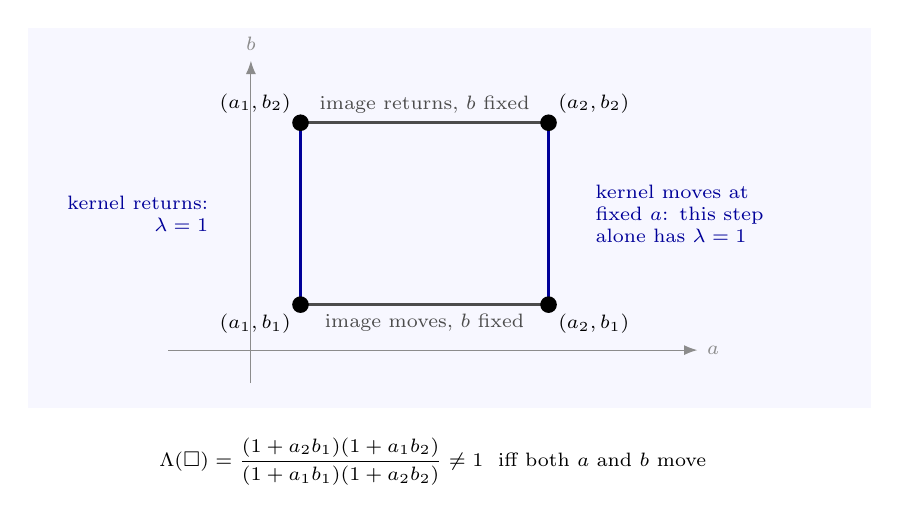
\begin{tikzpicture}[x=1.05cm,y=1.05cm,>=Latex,every node/.style={font=\scriptsize}]
  \fill[blue!3] (-2.7,-0.7) rectangle (7.5,3.9);
  \draw[->,black!45] (-1.0,0)--(5.4,0) node[right] {$a$};
  \draw[->,black!45] (0,-0.4)--(0,3.5) node[above] {$b$};
  \coordinate (v1) at (0.6,0.55);
  \coordinate (v2) at (3.6,0.55);
  \coordinate (v3) at (3.6,2.75);
  \coordinate (v4) at (0.6,2.75);
  \draw[very thick,black!70] (v1)--(v2);
  \draw[very thick,blue!60!black] (v2)--(v3);
  \draw[very thick,black!70] (v3)--(v4);
  \draw[very thick,blue!60!black] (v4)--(v1);
  \foreach \p/\lab/\pos in {v1/{(a_1,b_1)}/below left,
                            v2/{(a_2,b_1)}/below right,
                            v3/{(a_2,b_2)}/above right,
                            v4/{(a_1,b_2)}/above left}
    {\fill (\p) circle (3pt) node[\pos] {$\lab$};}
  \node[black!70,below] at (2.1,0.55) {image moves, $b$ fixed};
  \node[black!70,above] at (2.1,2.75) {image returns, $b$ fixed};
  \node[blue!60!black,align=left,anchor=west,text width=2.5cm] at (4.05,1.65)
    {kernel moves at fixed $a$: this step alone has $\lambda=1$};
  \node[blue!60!black,align=right,anchor=east] at (-0.4,1.65)
    {kernel returns:\\ $\lambda=1$};
  \node[align=center] at (2.2,-1.35)
    {$\Lambda(\square)=\dfrac{(1+a_2b_1)(1+a_1b_2)}{(1+a_1b_1)(1+a_2b_2)}\neq1$
     \ iff both $a$ and $b$ move};
\end{tikzpicture}
\caption[The four-step bivaluation square]%
{The four-step bivaluation square.  Each individual step has a corrected base
factor, but only the two image-moving steps contribute; the product is the
cross-ratio \eqref{eq:cross-ratio}.  A loop in which the kernel coordinate never
moves collapses to $\Lambda=1$ by Theorem~\ref{thm:no-radiation}.}
\label{fig:square}
\end{figure}

\subsection{An exact finite witness}

\begin{example}[$\F_7$ calibration]
\label{ex:f7}
Let $K=\F_7$, so that $|G|=336$, $|\Biv|=56$ and $|H|=6$ by Paper~IV,
Proposition~3.7 and Example~3.8.  Take the loop
\[
  (a_1,b_1)=(0,0),\quad (a_2,b_1)=(1,0),\quad (a_2,b_2)=(1,1),\quad (a_1,b_2)=(0,1).
\]
All four vertices are transverse, since $1+a_ib_j\in\{1,2\}\subset\F_7^\times$.
Then
\[
  \Lambda(\square)\equiv\frac{(1+0)(1+0)}{(1+0)(1+1)}\equiv 2^{-1}\equiv 4 \pmod 7,
\]
so $\Lambda(\square)=4\ne1$ in $H\cong\F_7^{\times}$.
\end{example}

This is the exact finite witness that the obstruction is not an artefact of the
real or complex topology: the holonomy is computed in a finite group of order
$336$, and it is a nonidentity element of the fiber $H$.  Appendix~\ref{app:matrices}
records the same example together with the exhaustive check of
\eqref{eq:projector-product} over all transverse loops in $\F_7$.

\subsection{The physical dictionary, stated as a dictionary}

\begin{warning}[What Hypothesis~\ref{hyp:radiation} adds]
\label{warn:radiation}
Theorem~\ref{thm:no-radiation} and Theorem~\ref{thm:cross-ratio} are theorems
about idempotents.  They say: a closed history whose kernel coordinate is
constant has a flat multiplicative transport, and a closed history that moves
both coordinates has a holonomy with an exact cross-ratio value.  They do not by
themselves say that anything is emitted.  The identification of
$\Lambda(\square)\ne1$ with radiation is Hypothesis~\ref{hyp:radiation}, and the
identification of its magnitude with radiated power is a further, unproved
refinement.

Three dictionary readings are available, and each should be judged on its own:
\begin{enumerate}[label=(\alph*)]
  \item \emph{Wavefront dislocation.}  The two pencils $\mathcal R_k$ and
  $\mathcal R_{k+1}$ are tangent at different ideal points, so at their interface
  the wavefronts cannot nest smoothly; the mismatch is a caustic, i.e. a kink in
  the propagating wavefront.  The magnitude of the mismatch is
  $|p_{k+1}-p_k|$ together with the holonomy $\Lambda$.
  \item \emph{Field falloff.}  In electrodynamics the field of an accelerated
  source has a term falling off as $1/r$ and proportional to the transverse
  acceleration, while the fields of static and uniformly moving sources fall off
  faster.  The correspondence asserted by Hypothesis~\ref{hyp:radiation} is that
  the non-telescoping holonomy is the \AEG{} carrier of that $1/r$ term.  No
  fall-off exponent is derived here.
  \item \emph{Phase residue.}  By Remark~\ref{rem:prequantum} the loop's
  non-closure along the Reeb fiber measures a phase; a phase that does not return
  to itself is the same kind of statement as a radiated quantum's escape.
\end{enumerate}
\end{warning}

\subsection{Relation to the \AEG{} manuscripts}

The construction proved in this section is not new to the \AEG{} series: it is
Paper~IV, Definition~4.10 and Theorem~4.11, with the $\F_7$ witness of
Example~4.13.  It was developed in the dialogue summarised here and recorded in
the manuscript under the heading of the projective-torsion problem.  The present
section's contribution is therefore not the theorem but the reading: the
non-telescoping holonomy of Paper~IV, Theorem~4.11 is the \AEG{} object
that the physical narrative calls ``radiation'', and
Corollary~\ref{cor:larmor} states the Larmor criterion in its terms.

Section~\ref{sec:torsion} completes the picture by packaging the same data into a
transport that also reproduces the affine torsion of Paper~0 on the Borel
sector.


\section{The Projective Torsion Transport}
\label{sec:torsion}
% ---------------------------------------------------------------------
% Section 7
% ---------------------------------------------------------------------

\begin{cnread}
上一节的 $\Lambda(\square)$ 是个「闭回路可观测量」，但它只是和乐，还不是一个
\emph{联络}。\AEG{} 手稿里的原始提法是：要一个规范等变的比较量，限制到
Borel 扇区 $B_\infty$ 时\textbf{退化回} Paper~0 的仿射平移挠率，而在闭回路上
又\textbf{不能被望远镜抵消}。本节把这两个要求在同一个对象里同时满足：把每条
历史边的算子步提升为半直积群 $\mathrm{Aff}(1,K)=K^\times\ltimes K$ 中的
\textbf{射影挠率传递元} $\mathcal T(e)=(\Lambda(e),\Delta\hat\xi(e))$。两个分量
一个管乘性曲率、一个管加性挠率，限制到 $b\equiv0$ 时前者归 $1$、后者一字不差
地退回 $\hat\xi_n$。本节同时指出附带的规范化因子 $2$ 问题（附录 B）。
\end{cnread}

\subsection{The problem, as \AEG{} states it}

Paper~IV, Section~13, lists as its first open problem:

\begin{quote}\small
\textbf{Projective torsion.}  Construct a gauge-equivariant comparison on
$G\to G/H$ that reduces to affine translation torsion in the Borel sector and
has a nontrivial closed-loop observable not forced to telescope \cite{AEG4}.
\end{quote}

Paper~IV, Proposition~4.9, explains why the naive attempt fails: if the edge
label of a lifted step is defined as the ratio $r_t=h_th_{t-1}^{-1}$ of vertex
frame lifts, then along every closed lifted path
$r_tr_{t-1}\cdots r_{s+1}=h_th_s^{-1}$ telescopes pairwise, so every closed path
has trivial product.  A nontrivial holonomy therefore requires the edge datum to
couple the base motion to the previous frame, not just to record the frames.

\subsection{The incidence-coupled transport}

The needed coupling is supplied by the projectors of
Theorem~\ref{thm:projector} without any additional structure: the natural pairing
between a new image point and the preceding kernel covector is
$\varphi_{b_{k-1}}(v_{a_k})=1+a_kb_{k-1}$.

\begin{definition}[Projective torsion transport,
{\cite[Def.~4.10]{AEG4}}]
\label{def:torsion-transport}
Let $K$ be a field, let $e_k:g_{k-1}\to g_k$ be a lifted step between regular
bivaluations with frame coordinates
\begin{equation}\label{eq:frame-lift}
  g_k=\begin{pmatrix}1&-a_k\\-b_k&1\end{pmatrix}
      \begin{pmatrix}\Phi_k&0\\0&1\end{pmatrix},
  \qquad \Phi_k\in K^{\times}\cong H,
\end{equation}
and suppose the step is transverse, $1+a_kb_{k-1}\ne0$.  The projective torsion
transport of $e_k$ is the element of the affine semidirect product
$\Aff(1,K)=K^{\times}\ltimes K$ given by
\begin{equation}\label{eq:torsion-transport}
  \mathcal T(e_k):=\begin{pmatrix}\Lambda_k&\Delta\hat\xi_k\\[2pt]0&1\end{pmatrix}
  \in\Aff(1,K),
\end{equation}
with multiplicative and additive components
\begin{equation}\label{eq:torsion-components}
  \Lambda_k=\frac{\Phi_k}{\Phi_{k-1}}\cdot\frac{1+a_kb_{k-1}}{1+a_{k-1}b_{k-1}}
  \in K^{\times},
  \qquad
  \Delta\hat\xi_k=-\Phi_{k-1}^{-1}\,\frac{a_k-a_{k-1}}{1+a_{k-1}b_{k-1}}\in K .
\end{equation}
The transport of a history $\gamma=(s_1,\dots,s_n)$ is the chronological
product $\mathcal T(\gamma)=\mathcal T(e_n)\cdots\mathcal T(e_1)$.
\end{definition}

Two remarks on the definition.  The first component generalises the base factor
\eqref{eq:lambda-edge} of Section~6 by multiplying it with the scale ratio of the
step; the second projects the image displacement onto the previous kernel
covector and normalises by the frame scale.  Both are forced once one asks that
the pair $(\Lambda,\Delta\hat\xi)$ be multiplicative along a history and
$\Aff(1,K)$-valued.

\subsection{The Borel reduction}

\begin{theorem}[Two checks, {\cite[Thm.~4.11]{AEG4}}]
\label{thm:torsion}
Let $\mathcal T$ be as in Definition~\ref{def:torsion-transport}.
\begin{enumerate}[label=(\alph*)]
  \item \emph{(Exact Borel reduction.)}  On the affine sector
  $B_\infty$, where $b_k\equiv0$ and $a_k=-\xi_k$ for every prefix
  $g_k(z)=\Phi_kz+\xi_k$, the base correction is identically $1$ and
  \begin{equation}\label{eq:borel-reduction}
    \Lambda_k\big|_{B_\infty}=\frac{\Phi_k}{\Phi_{k-1}}=s_k,
    \qquad
    \Delta\hat\xi_k\big|_{B_\infty}=\Phi_{k-1}^{-1}(\xi_k-\xi_{k-1}).
  \end{equation}
  Multiplying the matrices chronologically gives upper-left entry $\Phi_n$ and
  upper-right entry $\Phi_n\sum_k\Phi_k^{-1}(\xi_k-\xi_{k-1})=\xi_n$, which is
  the affine cocycle law of Paper~0, Proposition~7.1.  In particular, for two
  scale-compatible histories the translation component of
  $\mathcal T(\delta)^{-1}\mathcal T(\gamma)$ is exactly the relative affine
  defect $\Phi^{-1}(\xi_\gamma-\xi_\delta)$ of Paper~0, Section~7.4.
  \item \emph{(Non-telescoping holonomy off the sector.)}  On the four-step loop
  $\square$ of Theorem~\ref{thm:cross-ratio} with closed frame lift
  $\Phi_4=\Phi_0$, the multiplicative component of $\mathcal T$ reproduces
  $\Lambda(\square)$ of \eqref{eq:cross-ratio}.  Hence the transport has a
  closed-loop observable that is gauge-invariant and is not forced to telescope.
  \item \emph{(Modulated additive torsion.)}  Off $B_\infty$ the additive
  component carries the dynamic pole in its denominator, so the accumulated
  translation is a projective torsion modulated by the moving ripple pole rather
  than the affine one.
\end{enumerate}
\end{theorem}

\begin{proof}
(a) Put $b_k=0$ and $a_k=-\xi_k$ in \eqref{eq:torsion-components}: the factor
$(1+a_k\cdot0)/(1+a_{k-1}\cdot0)$ is $1$, leaving
$\Lambda_k=\Phi_k/\Phi_{k-1}$ and
$\Delta\hat\xi_k=-\Phi_{k-1}^{-1}(-\xi_k+\xi_{k-1})
=\Phi_{k-1}^{-1}(\xi_k-\xi_{k-1})$.  The matrix product of the
$\Aff(1,K)$-elements is
$\begin{pmatrix}\Phi_n&\Phi_n\sum\Phi_k^{-1}(\xi_k-\xi_{k-1})\\0&1\end{pmatrix}$,
and the sum telescopes to $\xi_n$ because $\xi_0=0$ (Paper~0,
Proposition~7.1).  (b) is Theorem~\ref{thm:cross-ratio}, whose gauge invariance
was proved there.  (c) is the presence of $1+a_{k-1}b_{k-1}$ in the denominator
of $\Delta\hat\xi_k$, which is not a function of the charges alone once
$b\ne0$.
\end{proof}

\begin{remark}[Why the two demands can be met at once]
\label{rem:two-demands}
The Borel reduction of part (a) and the non-telescoping holonomy of part (b) look
like competing requirements, because a quantity that is multiplicative and
vanishes on $b\equiv0$ might be expected to vanish identically.  They coexist
because they live in different components of $\Aff(1,K)$: the reduction uses the
additive component (the translation $\Delta\hat\xi$, which becomes the affine
cocycle), while the obstruction uses the multiplicative component (the cross
ratio).  On the Borel sector the multiplicative component degenerates to the
step's own scale ratio, which telescopes as it must; off it, the same component
carries the extra base factor and does not.
\end{remark}

\subsection{The curvature of the transport}

For $K=\R$ or $\CC$ one can pass to the infinitesimal picture.  Paper~IV,
Remark~4.12, records the reductive connection whose solder component and
connection one-form are
\begin{equation}\label{eq:connection}
  \omega_H=\Phi^{-1}\mathrm d\Phi+\frac{a\,\mathrm db-b\,\mathrm da}{1+ab},
  \qquad
  \theta_+=\frac{\Phi^{-1}\mathrm da}{1+ab},
\end{equation}
and it records two facts about them that were stated loosely in an earlier
version of that remark and are now exact.  First, its curvature is
$2(1+ab)^{-2}\mathrm da\wedge\mathrm db$, twice the para-K\"ahler form; the
first-order transport density of the cross-ratio holonomy is that form with a
minus sign, so the transport is the holonomy of the connection whose transverse
part is halved (Paper~IV, Proposition~4.17).  Second, on the Borel sector the
solder component evaluates to
\begin{equation}\label{eq:solder-borel}
  \theta_+\big|_{b=0}=\Phi^{-1}\mathrm da=-e^{-M}\mathrm d\xi ,
\end{equation}
because the image coordinate satisfies $a=-\xi$ there; this is \emph{minus} the
left Maurer--Cartan translation form $e^{-M}\mathrm d\xi$ of Paper~0,
Proposition~7.4, Equation~(60).  The minus sign is the sign of $a=-\xi$, not a
different convention for the connection.

The comparison of the two densities is Lemma~\ref{lem:factor-two}.

\begin{lemma}[Two densities, one factor]
\label{lem:factor-two}
The curvature of the connection \eqref{eq:connection} is
$\mathrm d\omega_H=2(1+ab)^{-2}\mathrm da\wedge\mathrm db$, whereas the
first-order log-holonomy density of Corollary~\ref{cor:larmor} is
$-(1+ab)^{-2}\mathrm da\wedge\mathrm db$.  The two differ by the factor $-2$ and
by the choice of orientation.
\end{lemma}

\begin{proof}
Since the $\Phi$-term of $\omega_H$ is closed, only
$\omega_2=(1+ab)^{-1}(a\,\mathrm db-b\,\mathrm da)$ contributes.  With
$f=(1+ab)^{-1}$ one has $\mathrm d\omega_2=\bigl(\partial_a(fa)+\partial_b(fb)
\bigr)\mathrm da\wedge\mathrm db$, and
$\partial_a(fa)+\partial_b(fb)=-2ab(1+ab)^{-2}+2(1+ab)^{-1}=2(1+ab)^{-2}$.  The
transport density is Corollary~\ref{cor:larmor}.  Check~V4.1 verifies the
coefficient symbolically.
\end{proof}

\begin{remark}[Status of the factor]
\label{rem:factor-two}
Lemma~\ref{lem:factor-two} is a normalisation observation, not a contradiction:
the cross-ratio formula \eqref{eq:cross-ratio} is exact and verified, and the
curvature statement of the manuscript is exact as a statement about
\eqref{eq:connection}.  The two normalisations differ by $2$ because the
transport of Definition~\ref{def:torsion-transport} is the holonomy of
$\tfrac12$ of the connection's solder--connection split, i.e. of a connection
whose second term carries a factor $\tfrac12$.  Any statement that identifies
the radiated power with a curvature integral must therefore fix this
normalisation first.  Appendix~\ref{app:curvature} records the computation.

A second observation, unrelated to the factor: three cross-references inside
Paper~IV, Subsection~4.10--4.13 (\texttt{ex:f7-counts},
\texttt{prop:telescoping}, \texttt{eq:chart-projector}) resolved to
\texttt{??} in the build of 20 October 2026, because those labels did not exist.
They have since been repaired in the manuscript source --- the example of
Subsection~3.6 is now labelled, and the other two references point to
Proposition~4.9 and to the projector display \eqref{eq:projector} --- and the
rebuilt Paper~IV reports no undefined reference.
Appendix~\ref{app:register} records the repair together with a second, smaller
one in Paper~0.
\end{remark}

\subsection{The finite witness, restated}

Example~\ref{ex:f7} applies verbatim to the transport: on
$K=\F_7$ with the loop $\square$ taking
$(0,0)\to(1,0)\to(1,1)\to(0,1)\to(0,0)$ and $\Phi_k\equiv1$, one gets
$\Lambda(\square)=4=2^{-1}\in\F_7^{\times}$, a nonidentity element of
$H$.  With $\Phi_k\equiv1$ the additive components are
$\Delta\hat\xi_k=-(a_k-a_{k-1})/(1+a_{k-1}b_{k-1})$, so the transport is a purely
finite, exactly computable object.  Appendix~\ref{app:matrices} lists the four
edge transports of this loop explicitly.

\subsection{Where this leaves the open problem}

Theorem~\ref{thm:torsion} supplies both demands of the problem statement: the
transport reduces exactly to affine torsion on $B_\infty$, and off $B_\infty$ it
has a closed-loop observable that is gauge-invariant and provably not forced to
telescope, with a finite witness.  What the theorem does not supply is a
physical calibration of the transport's \emph{units}: no statement is made about
which physical quantity $\Lambda(\square)-1$ measures, beyond the dictionary of
Hypothesis~\ref{hyp:radiation}.  That is the open end recorded in
Section~\ref{sec:summary}.


\section{Dynamical Scattering: M\o ller and Bhabha Sectors}
\label{sec:scattering}
% ---------------------------------------------------------------------
% Section 8
% ---------------------------------------------------------------------

\begin{cnread}
两个带电粒子「带着动量碰撞」在 \AEG{} 里对应什么？本节给出一个纯代数的
区分：$e^-e^-$ 散射（M\o ller）只有 $t$-道与 $u$-道，两者都留在仿射扇区
$B_\infty$ 内；而 $e^+e^-$ 散射（Bhabha）多出一条 $s$-道，它在 \AEG{} 中
恰好是\textbf{跨越 Bruhat 大胞腔}：$\PGL_2=B_\infty\sqcup B_\infty JB_\infty$
（Paper~0 公式 47），必经一次反演 $J(z)=-1/z$。总加法荷归零（$+e-e=0$）
正是「分母归零」的代数来源，而射影延拓让人从 $z=0$ 穿到 $\infty$。
这里要提醒：这是\textbf{结构对应}，不是振幅的推导。
\end{cnread}

\subsection{Two electrons: both channels inside the affine sector}

Let both particles be electrons.  Then the total additive charge of any history
containing both is $-2e\ne0$, so no closed charge loop and hence no annihilation
channel exists: by Proposition~\ref{prop:dipole-loop} the closed-loop mechanism
requires opposite charges.

Two histories remain, and both are affine.

\begin{enumerate}[label=(\roman*)]
  \item \emph{Threading order.}  The word exchanges one quantum while the two
  world lines keep their order in the scale coordinate; this is the
  ``$t$-channel'' history of the exchange, and it is a word in
  $B_\infty$ whose total charge is $(-e,\,-e)$.
  \item \emph{Crossed order.}  The two final-state world lines are exchanged, so
  the appropriate comparison is between two histories $\gamma$ and $\delta$
  whose scale steps are interleaved; this is the ``$u$-channel'' of identical
  particles, and by Theorem~8.9 of Paper~0 the relative defect is the weighted
  area between the two charge chains.
\end{enumerate}

In both cases the surviving velocity dependence is the one computed in
Proposition~\ref{prop:ampere}: the two histories differ in their direction angle
$\theta_1-\theta_2$, and the pairing gives the coefficient
$1-\mathbf v_1\!\cdot\!\mathbf v_2/c^{2}$ relative to the Coulomb term.  For
collinear motion this is the correction computed in
Corollary~\ref{cor:parallel-currents}.

\begin{remark}[On spin]
\label{rem:spin}
A spin-$\tfrac12$ charge would need the double cover of the projective group, i.e.
the passage from $\PSL_2(\C)$ to $\SL_2(\C)$, whose two-dimensional
representation is generated by the Pauli matrices.  Nothing in Paper~0 or
Paper~IV supplies that cover, and no spin-dependent statement is proved in this
note.  The remark is recorded because the physical narrative contains it.
\end{remark}

\subsection{Electron and positron: the second Bruhat cell}

Now let the particles be an electron and a positron.  Two of the three channels
are affine, and one is not.

\begin{enumerate}[label=(\roman*)]
  \item \emph{Exchange without annihilation.}  The ``$t$-channel'' photon
  exchange is the configuration of Section~\ref{sec:coulomb}: a bound-state
  history in $B_\infty$ with potential $V=-\alpha_e/r$ and defect
  $e(1-e^{-M_*})$ by Proposition~\ref{prop:dipole-loop}.
  \item \emph{Annihilation.}  At high relative momentum the pair acquires a
  channel with no like-charge analogue.  Its algebraic signature is that the
  total additive charge vanishes, $A_{\mathrm{tot}}=(+e)+(-e)=0$, exactly as in
  the closed loop of Proposition~\ref{prop:dipole-loop}.
  \item \emph{Regeneration.}  The word then continues from the vanishing
  denominator, and the projective continuation of Paper~0, Section~5.1 carries
  it through infinity and back to a finite pair.
\end{enumerate}

The third item is where the projective cell is entered, and \AEG{} has an exact
statement about it.

\begin{theorem}[Bruhat decomposition, {\cite[Eq.~(47) and Thm.~6.2]{AEG0}}]
\label{thm:bruhat}
For any field $K$,
\begin{equation}\label{eq:bruhat}
  \PGL_2(K)=B_\infty\sqcup B_\infty J B_\infty,
\end{equation}
and every $F\in\PGL_2(K)$ with nonzero lower-left entry admits the exact
factorization
\begin{equation}\label{eq:factorization}
  F=T_{A/C}\circ D_{(AD-BC)/C^{2}}\circ J\circ T_{D/C},
\end{equation}
i.e. translate, scale, invert, translate.  The first cell consists of operators
whose pole is infinity; the second consists of operators with a finite pole in
the chosen affine chart.
\end{theorem}

\begin{proof}
Paper~0, Theorem~6.2 and its proof; the two cases $C=0$ and $C\ne0$ are
$F=T_{B/D}\circ D_{A/D}$ and \eqref{eq:factorization} respectively.
\end{proof}

The reading of the theorem in the scattering picture is now a translation of its
two displayed statements: a history that stays in $B_\infty$ has a pole at
infinity, and a history that produces a finite pole must contain the inverting
element exactly once.

\begin{center}\small
\renewcommand{\arraystretch}{1.25}
\begin{tabular}{@{}p{0.2\linewidth}p{0.24\linewidth}p{0.24\linewidth}p{0.24\linewidth}@{}}
\toprule
process & charges & \AEG{} sector & mechanism \\
\midrule
$e^-e^-\to e^-e^-$ & $(-e,-e)$, $A_{\mathrm{tot}}=-2e\ne0$
& $B_\infty$ only & threading and crossed (identical-particle) orders; no closed
charge loop \\
$e^+e^-\to e^+e^-$ & $(-e,+e)$, $A_{\mathrm{tot}}=0$
& $B_\infty$ and $B_\infty JB_\infty$ & exchange, plus a channel that must cross
$J$ because the total additive charge vanishes \\
$(e^-e^-)$ emission & $(-e,-e)$ & $B_\infty$, pole jumps
& radiation as in Section~\ref{sec:radiation}: the pole may move inside the
affine cell \\
\bottomrule
\end{tabular}
\end{center}

\subsection{What the correspondence does and does not assert}

\begin{warning}[Structural, not dynamical]
\label{warn:scattering}
The table above is a correspondence between channel types and Bruhat cells.  It
is not a derivation of a scattering amplitude, a cross section, or a Feynman rule
for the annihilation channel.  In particular:
\begin{enumerate}[label=(\alph*)]
  \item The vanishing of $A_{\mathrm{tot}}$ is an exact statement about charges
  (Theorem~8.6); the statement that a physical annihilation requires it is a
  dictionary statement.
  \item The projective continuation through an inadmissible division is exact in
  \AEG{} (Paper~0, Section~5.1) but says nothing about which intermediate states
  are kinematically allowed.  Ordinary division by zero remains inadmissible;
  what the continuation supplies is a value at the pole, not a physical process.
  \item The separation ``$t$-channel inside $B_\infty$, $s$-channel across
  $B_\infty JB_\infty$'' is a two-cell statement.  A quantitative Bhabha cross
  section would require a measure on histories, i.e. the path-integral structure
  of Remark~\ref{rem:prequantum}, which is not constructed here.
\end{enumerate}
\end{warning}

What survives is the qualitative separation, and it is not empty: it explains why
the like-charge and unlike-charge cases must differ in \emph{kind} rather than
only in sign, and it locates the difference in an exact algebraic invariant (the
Bruhat cell of the composite) rather than in the sign of a coupling.


\section{Bound States: Closed Loops and Bohr--Sommerfeld Quantization}
\label{sec:bohr}
% ---------------------------------------------------------------------
% Section 9
% ---------------------------------------------------------------------

\begin{cnread}
电动力学的另一面是束缚态：正负电荷若既有吸引、又有切向运动，就既不湮灭
也不逃逸，而是形成周期轨道。在 \AEG{} 里这正是\textbf{椭圆型}不动点：连续
分数迭代 $z_{k+1}=E-e^2/z_k$ 的判别式 $E^2-4e^2<0$ 时，两个不动点落在
上半平面内部的共轭复点上，算子变成旋转。把这条闭合轨道水平提升到切触空间，
它绕一圈不闭合，而是沿着 Reeb 纤维漂移 $\Delta A=-\oint a\,dM$。把这个漂移
取成基本作用量的整数倍（Boothby--Wang 预量化），就得到玻尔--索末菲条件，
代入库仑势直接给出 $E_n=-\dfrac{m\alpha_e^2}{2\hbar^2 n^2}$。本节末尾说明
这一推导的\textbf{半经典}身份。
\end{cnread}

\subsection{Hyperbolic, parabolic, and elliptic histories}

A projective motion $F\in\PSL_2(\R)$ is classified by its fixed-point set, and by
Paper~0, Subsection~5.5, the finite fixed points solve
\begin{equation}\label{eq:mobius-fixed}
  Cz^{2}+(D-A)z-B=0 .
\end{equation}

\begin{enumerate}[label=(\roman*)]
  \item \emph{Hyperbolic}: two distinct real fixed points.  The motion is a
  translation along the geodesic joining them; in the flow \eqref{eq:theta-flow}
  the scale coordinate advances monotonically.  A pair of charges in radial
  infall or escape follows this type.
  \item \emph{Parabolic}: one double fixed point, necessarily on the boundary.
  The corresponding motion is the horocyclic translation $\mathsf X_s$ of
  \eqref{eq:grid-motions}.
  \item \emph{Elliptic}: two complex conjugate fixed points in
  $\CC\setminus\R$, i.e. inside $\HH^2$ when read in the upper half-plane model.
  The motion is conjugate to a rotation, and its orbit is a closed curve around
  the interior fixed point.  A bound two-body motion follows this type.
\end{enumerate}

The Coulomb problem supplies the elliptic case through the continued-fraction map
of Paper~0, Subsection~5.4.  There, the stationary right-reciprocal update is
$F(z)=a+b/z$ with matrix $M_F=\begin{pmatrix}a&b\\1&0\end{pmatrix}$ and fixed
points $z^{2}-az-b=0$.  Writing the bound-state iteration as
\begin{equation}\label{eq:coulomb-iteration}
  z_{k+1}=E-\frac{e^{2}}{z_k},
  \qquad
  M_F=\begin{pmatrix}E&-e^{2}\\1&0\end{pmatrix},
\end{equation}
the fixed-point equation becomes $z^{2}-Ez+e^{2}=0$, whose discriminant is
$\Delta=E^{2}-4e^{2}$.  For $E<2e$ the discriminant is negative, the two fixed
points are complex conjugates, and the motion is elliptic.

\begin{remark}[Status of the continued fraction]
\label{rem:cf-status}
Equation~\eqref{eq:coulomb-iteration} is the algebraic statement of Paper~0,
Subsection~5.4 with $(a,b)=(E,-e^{2})$.  Its identification with the spectral
problem of a Coulomb Hamiltonian is a dictionary statement, not a theorem: what
\AEG{} supplies is the conjugacy classification of the iteration, and what the
dictionary supplies is the assertion that the physical bound states sit at the
parameter values where that classification becomes elliptic.
\end{remark}

\subsection{The Reeb holonomy of a closed orbit is the action}

Let $\gamma_{\mathrm{orb}}$ be a closed orbit of a bound motion in
$\HH^2_{(M,a)}$, and let $\tilde\gamma_{\mathrm{orb}}$ be its horizontal lift to
$\Cont$.  By Theorem~\ref{thm:dual-tearing}(2) the lift does not close in
$\Cont$: it ends at a Reeb height differing from its starting height by
\begin{equation}\label{eq:orbit-holonomy}
  \Delta A(\gamma_{\mathrm{orb}})
  =-\oint_{\gamma_{\mathrm{orb}}}a\,\mathrm dM
  =-\iint_{\Omega_{\mathrm{orb}}}\mathrm da\wedge\mathrm dM ,
\end{equation}
where $\Omega_{\mathrm{orb}}$ is the region enclosed by the orbit in the
$(M,a)$-plane.

\begin{lemma}[The action slot]
\label{lem:action-slot}
Assume Hypothesis~\ref{hyp:depth} and let the assignment slot of the contact
form be filled by the scale-corrected radial momentum, $a:=r\,p_r$.  Then
\begin{equation}\label{eq:action-form}
  -\oint a\,\mathrm dM=-\oint p_r\,\mathrm dr ,
\end{equation}
so that the Reeb drift \eqref{eq:orbit-holonomy} is minus the classical
mechanical action of the orbit.
\end{lemma}

\begin{proof}
$M=\log(r/\ell_0)$ gives $\mathrm dM=\mathrm dr/r$, hence
$a\,\mathrm dM=r p_r\,\mathrm dr/r=p_r\,\mathrm dr$; the sign is the orientation
of the loop.
\end{proof}

\begin{warning}[What the substitution assumes]
\label{warn:action-slot}
Lemma~\ref{lem:action-slot} is the point at which the note departs from purely
\AEG{} statements: the assignment of the contact form is a number attached to a
history, and calling it $r p_r$ --- with $r$ the physical separation --- is a
dictionary step additional to Hypotheses~\ref{hyp:charge}--\ref{hyp:pairing}.  It
is however the least avoidable one, because without it the Reeb drift is a
dimensionless area and cannot be compared with $\hbar$.
\end{warning}

\subsection{Monodromy and the Bohr--Sommerfeld condition}

Suppose the Reeb fiber is compactified.  By the Boothby--Wang theorem
\cite{BoothbyWang1958,Geiges2008}, if the contact form's Reeb field is a
circle action with period $2\pi\hbar$, then $\Cont$ is the total space of a
principal $S^{1}$-bundle --- the prequantum bundle of the underlying symplectic
manifold $\HH^2$ --- and the horizontal lift of a closed orbit closes in the
fiber exactly when its drift is an integer multiple of the period.

\begin{definition}[Monodromy condition]
\label{def:monodromy}
The quantized contact model is the quotient $\Cont/(2\pi\hbar\,\mathbb Z\cdot R)$
of the Reeb flow.  A closed orbit $\gamma_{\mathrm{orb}}$ defines a monodromy
element $\exp(\mathrm i\,\Delta A(\gamma_{\mathrm{orb}})/\hbar)\in S^{1}$, and it
defines a single-valued state exactly when
\begin{equation}\label{eq:bohr-sommerfeld}
  \oint_{\gamma_{\mathrm{orb}}}(-a\,\mathrm dM)
  =\oint p_r\,\mathrm dr
  =2\pi n\hbar ,
  \qquad n\in\mathbb Z .
\end{equation}
\end{definition}

\begin{theorem}[Coulomb spectrum]
\label{thm:spectrum}
Under Hypothesis~\ref{hyp:charge}--\ref{hyp:pairing}, Lemma~\ref{lem:action-slot},
and Definition~\ref{def:monodromy}, the bound orbits of a Coulomb pair in the
radial coordinate satisfy
\begin{equation}\label{eq:radial-action}
  \oint p_r\,\mathrm dr
  =2\pi\Bigl(\frac{m\alpha_e}{\sqrt{-2mE}}-l\Bigr)=2\pi n_r\hbar ,
\end{equation}
with $\alpha_e=e^{2}/(4\pi)$ and $l$ the angular momentum.  Writing
$n=n_r+l/\hbar$, the energies are
\begin{equation}\label{eq:spectrum}
  E_n=-\frac{m\alpha_e^{2}}{2\hbar^{2}n^{2}},
  \qquad n=1,2,3,\dots
\end{equation}
\end{theorem}

\begin{proof}
The second equality in \eqref{eq:radial-action} is the standard Coulomb radial
action; Appendix~\ref{app:action} evaluates the half-action
$\int_{r_-}^{r_+}p_r\,\mathrm dr=\pi\bigl(m\alpha_e/\sqrt{-2mE}-l\bigr)$ both
in closed form and by numerical quadrature at three parameter points
(Checks~V7.1).  Dividing by $2\pi\hbar$ and putting $n_r=n-l/\hbar$ gives
$m\alpha_e/\sqrt{-2mE}=\hbar n$, hence $-2mE=m^{2}\alpha_e^{2}/(\hbar^{2}n^{2})$
and \eqref{eq:spectrum}.  Check~V7.2 verifies the quantization condition and
Check~V7.3 the ground-state value.
\end{proof}

\begin{remark}[The residue picture]
\label{rem:residue}
The integral \eqref{eq:radial-action} is a contour integral between the two
turning points, i.e. between the two real roots of the quadratic that Paper~0,
Proposition~5.4 attaches to the iteration.  Its closed form is the residue
difference between the two ends of the contour.  In the bivaluation language of
Section~\ref{sec:radiation} the two ends are the two punctures
$(q^+,q^-)=(0,\infty)$ of the reference pair, so the same integral is a residue
pairing at the two ends of the frame.  This is a suggestive identification, not a
proof; it is recorded because it is the natural continuation of the present
picture.
\end{remark}

\subsection{How semiclassical is this?}

\begin{warning}[Range of the derivation]
\label{warn:semiclassical}
Theorem~\ref{thm:spectrum} is a Bohr--Sommerfeld (EBK) computation, not a
solution of the Schr\"odinger equation.  Three limitations should be stated.
\begin{enumerate}[label=(\alph*)]
  \item The condition \eqref{eq:bohr-sommerfeld} quantizes a single action
  integral; a genuine quantization would need the full polarization and the
  half-form (metaplectic) correction of geometric quantization.  For the Coulomb
  problem those corrections are known to conspire so that the leading
  Bohr--Sommerfeld spectrum is exact, but that is a property of this particular
  potential, not a consequence of the present construction.
  \item The Langer-type correction $l\mapsto l+\tfrac12$ changes the spectrum
  beyond leading order; no statement about it is made here.
  \item Nothing above defines a Hilbert space, an inner product, or an operator
  algebra.  The Reeb circle of Definition~\ref{def:monodromy} is a compactification
  hypothesis, and the multiplicities of the resulting levels are not counted.
\end{enumerate}
What the section does establish is narrower and exact: the quantity that
Bohr--Sommerfeld quantizes is, in this picture, the Reeb drift of a closed
horizontal loop --- an object that exists in \AEG{} independently of any physical
reading --- and the Coulomb input enters only through
Lemma~\ref{lem:action-slot} and the classical integral of
Theorem~\ref{thm:spectrum}.
\end{warning}


\section{Dictionary, Status Ledger, and Open Ends}
\label{sec:summary}
% ---------------------------------------------------------------------
% Section 10
% ---------------------------------------------------------------------

\begin{cnread}
本节把全篇收拢成三张表：\textbf{对照表}（物理概念 $\leftrightarrow$
\AEG{} 对象 $\leftrightarrow$ 出处）、\textbf{状态账}（每条结论依赖哪几条
字典假设）、以及\textbf{开放端}（哪些地方本稿只是对应、不是推导）。
一句话总结：\AEG{} 提供了「荷、标度、切触曲率、交叉比和乐、Reeb 漂移、
径向作用量」这套确切的数学；物理电动力学要靠四条（严格说五条）字典假设才
接得上，接上之后库仑、安培、辐射、束缚态四件事的\textbf{符号与结构}都能
读出来，但\textbf{数值标定}（尤其是辐射功率与 $\hbar$ 的单位）仍是空的。
\end{cnread}

\subsection{The dictionary}

{\small
\renewcommand{\arraystretch}{1.22}%
\begin{longtable}{@{}p{0.235\linewidth}p{0.335\linewidth}p{0.365\linewidth}@{}}
\toprule
physical notion & \AEG{} object & reference and status \\
\midrule
\endfirsthead
\toprule
physical notion & \AEG{} object & reference and status \\
\midrule
\endhead
\midrule
\multicolumn{3}{r}{\emph{continued}}\\
\endfoot
\bottomrule
\endlastfoot
asymptotic (bare) state & ideal point $q\in\pt_\infty\HH^2$
& Paper~0, \S\S 3--4; dictionary \\
dressed state at scale $r$ & ordinary point $p$ with $y_p=e^{-M_*}$
& Prop.~\ref{prop:operator-fiber}; dictionary \\
scale evolution & multiplicative motion $\cM_m$, $M=\lambda v$
& Prop.~3.6, Thm.~8.6 \\
virtual quantum emission & additive motion $\cA_t$ at depth $M_i$
& Eq.~\eqref{eq:comb-cocycle}; Hyp.~\ref{hyp:charge} \\
charge of a particle & sign of the additive step; positron $=\mathcal R$
conjugate
& Lemma~\ref{lem:reflection}; Hyp.~\ref{hyp:charge} \\
sum over diagrams & the fiber $\rho^{-1}(g_{p_0\to p})$
& Prop.~\ref{prop:operator-fiber}; exact \\
bare coupling divergence & abscissa $A_\gamma$ of the \ACS{}
& Cor.~\ref{cor:bare-divergence}; exact \\
renormalisation cancellation & vanishing weighted area
$\tau(\gamma,\delta)$
& Thm.~8.9; exact \\
path-integral phase & Reeb height $u_\gamma=A_\gamma/\mu$
& Prop.~\ref{prop:reeb-heights}, Rem.~\ref{rem:prequantum}; exact object,
dictionary reading \\
electrostatic potential & $a_1(r)=q_1e^{-M_*}$
& Eq.~\eqref{eq:field-at-2}; Hyps.~\ref{hyp:charge}, \ref{hyp:depth} \\
Coulomb sign rule & sign of $\kappa=\mu\lambda\propto q_1q_2$
& Eq.~\eqref{eq:kappa}; Hyps.~\ref{hyp:charge}--\ref{hyp:pairing} \\
binding energy of a dipole & $\tau(\ell,\varnothing)=e(1-e^{-M_*})$
& Prop.~\ref{prop:dipole-loop}; Hyp.~\ref{hyp:pairing} \\
motion (velocity) & direction angle $\theta$, tilt $\mathrm dM/\mathrm d\tau$
& Thm.~3.9; Hyp.~\ref{hyp:velocity} \\
Amp\`ere force & one-form pairing $\alpha_1(\dot\gamma_2)$
& Prop.~\ref{prop:ampere}; Hyps.~\ref{hyp:velocity}, \ref{hyp:pairing} \\
frame compression by a boost & hyperbolic element $D_{e^\eta}\in H$ on the
pencil
& Thm.~4.2, Paper~IV Thm.~3.5; exact object \\
Lorentz signature & indefinite Killing form of $\mathfrak{sl}_2$
& Lemma~\ref{lem:killing}; exact \\
no radiation of uniform motion & $\Lambda=1$ for constant kernel coordinate
& Thm.~\ref{thm:no-radiation}; exact, read via Hyp.~\ref{hyp:radiation} \\
radiation of acceleration & $\Lambda(\square)\ne1$ for moved kernel coordinate
& Thm.~\ref{thm:cross-ratio}; exact, read via Hyp.~\ref{hyp:radiation} \\
sector of annihilation & Bruhat cell $B_\infty JB_\infty$
& Thm.~\ref{thm:bruhat}; exact object, dictionary reading \\
bound state & elliptic element; closed orbit inside $\HH^2$
& Prop.~5.4, \S 5.5; exact object \\
action of a bound orbit & Reeb drift $-\oint a\,\mathrm dM$
& Thm.~\ref{thm:dual-tearing}; Lemma~\ref{lem:action-slot} \\
quantization & monodromy on the compactified Reeb circle
& Def.~\ref{def:monodromy}; semiclassical \\
\end{longtable}}

\subsection{Status ledger}

{\small
\renewcommand{\arraystretch}{1.22}%
\begin{longtable}{@{}p{0.44\linewidth}p{0.24\linewidth}p{0.26\linewidth}@{}}
\toprule
conclusion & hypotheses needed & confidence \\
\midrule
\endfirsthead
\toprule
conclusion & hypotheses needed & confidence \\
\midrule
\endhead
\midrule
\multicolumn{3}{r}{\emph{continued}}\\
\endfoot
\bottomrule
\endlastfoot
the $p_0\to p$ family is one operator fiber & none & theorem \\
the same family fans out in $\ACS$ with a weighted constraint & none & theorem \\
the two projections are Legendre-conjugate, with $\Delta a$ versus $\Delta A$
& none & theorem (Paper~0, Thm.~9.9) \\
the kernel word realizes $p(1-e^{-q})$ three ways & none & theorem + check \\
$\kappa$ changes sign exactly when one charge does & Hyp.~\ref{hyp:pairing}
& sign structure is exact; magnitude is dictionary \\
like charges repel, unlike attract & Hyps.~\ref{hyp:charge}--\ref{hyp:pairing}
& conditional; sign rule robust \\
the neutral pair has binding defect $e(1-e^{-M_*})$
& Hyp.~\ref{hyp:pairing} & conditional \\
$F=\frac{q_1q_2}{4\pi r^2}\bigl(1-\mathbf v_1\!\cdot\!\mathbf v_2/c^2\bigr)$
& Hyps.~\ref{hyp:charge}--\ref{hyp:velocity} & conditional; equals the Darwin
coefficient \\
parallel currents attract the two electrons & same & conditional \\
uniform motion is non-radiative & Hyp.~\ref{hyp:radiation} & algebraic part: theorem \\
acceleration produces a non-telescoping holonomy & Hyp.~\ref{hyp:radiation}
& algebraic part: theorem; with an $\F_7$ witness \\
radiated power $\propto\Lambda-1$ & Hyp.~\ref{hyp:radiation}
& \emph{open}: no calibration \\
M\o ller inside $B_\infty$, Bhabha across $B_\infty JB_\infty$
& Hyps.~\ref{hyp:charge}, \ref{hyp:pairing} & correspondence only \\
Bohr--Sommerfeld spectrum $E_n=-m\alpha_e^{2}/(2\hbar^{2}n^{2})$
& all five + Lemma~\ref{lem:action-slot} & semiclassical, exact for Coulomb \\
\end{longtable}}

\subsection{What is exact and what is not}

Three groups should be kept apart.

\paragraph{Exact \AEG{} mathematics used here.}
The operator fiber of Proposition~\ref{prop:operator-fiber}; the fan-out and the
weighted constraint of Proposition~\ref{prop:acs-fanout}; the Legendre
conjugacy of Theorem~\ref{thm:dual-tearing} (Paper~0, Theorem~9.9); the three
evaluations of the kernel word; the reflection conjugation of
Lemma~\ref{lem:reflection}; the orientation reversal of
Lemma~\ref{lem:orientation} (Paper~0, Appendix~D.1); the closed dipole loop
(Paper~0, Appendix~D.2); the no-radiation and cross-ratio theorems of
Section~\ref{sec:radiation} with the $\F_7$ witness; the Borel reduction and
non-telescoping holonomy of Theorem~\ref{thm:torsion} (Paper~IV,
Theorem~4.11); the Bruhat decomposition and factorization
(Paper~0, Theorem~6.2); the Kepler conjugation classification
(Paper~0, Proposition~5.4, Subsection~5.5); and the radial action
computation of Appendix~\ref{app:action}.

\paragraph{Declared dictionaries.}
Hypotheses~\ref{hyp:charge}--\ref{hyp:velocity}.  Each names a physical
quantity by an \AEG{} object.  They are not proved, not provable inside \AEG{},
and not claimed.

\paragraph{Heuristics used for orientation only.}
(i) The ``opening spring'' and ``annihilating composition'' pictures of
Section~\ref{subsec:three-readings}; (ii) the relative-shear reading of the
$v\to c$ limit in Remark~\ref{rem:v-to-c}; (iii) the wavefront-caustic reading of
the holonomy in Warning~\ref{warn:radiation}; (iv) the residue-pairing remark of
Remark~\ref{rem:residue}; (v) the spin remark of Remark~\ref{rem:spin}.  These
are explanatory devices.  They are marked in place, and no conclusion rests on
them.

\subsection{Open ends}

\begin{problem}[A three-dimensional carrier]
Every force law quoted here carries the factor $4\pi$ imported from the solid
angle of three-space.  The \AEG{} carriers used are one-dimensional in the
multiplicative direction and two-dimensional in the contact model.  What is
required is an \AEG{} model whose multiplicative direction is genuinely
three-dimensional, so that the $1/r$ kernel and the $4\pi$ normalisation are
computed rather than inserted.
\end{problem}

\begin{problem}[Units of the radiation observable]
Theorem~\ref{thm:cross-ratio} produces a number $\Lambda(\square)-1$ from a
history, and Hypothesis~\ref{hyp:radiation} calls it radiation.  No statement
converts it into a power.  A calibration would need either (a) a variational
principle on histories whose second variation reproduces the Larmor rate, or
(b) an identification of $\log\Lambda$ with a phase whose derivative is an energy
flux.  Neither is available.  The factor-two normalisation of
Lemma~\ref{lem:factor-two} must be settled first.
\end{problem}

\begin{problem}[A measure on the operator fiber]
Proposition~\ref{prop:operator-fiber} identifies the sum over diagrams with a
fiber of an evaluation map, and Remark~\ref{rem:prequantum} identifies a
candidate phase.  A genuine path integral needs a measure on the fiber that is
invariant under the frame changes of Paper~IV, Theorem~3.5.  Whether the Reeb
length $e^{-M}\mathrm dA$ of Paper~0, Proposition~8.2, is the right
quasi-invariant measure is open.
\end{problem}

\begin{problem}[Spin]
Remark~\ref{rem:spin}: the double cover $\SL_2(\C)\to\PSL_2(\C)$ and its
two-dimensional representation are not part of the \AEG{} structure used here.
A spin-dependent force or a spin-statistics statement would require extending
the frame torsor of Paper~IV to the metaplectic cover.
\end{problem}

\begin{problem}[Beyond the Darwin order]
Warning~\ref{warn:darwin}: the coefficient of
Proposition~\ref{prop:ampere} is the $O(v^{2}/c^{2})$ term.  Whether the contact
picture can produce the full velocity dependence --- and, if so, whether the
indefinite structure of Lemma~\ref{lem:killing} is the mechanism --- is open.
\end{problem}

\subsection{Closing remark}

The five working notes that this document consolidates were an exploration, and
the exploration found something worth stating precisely: the same order defect
that \AEG{} proves to be a weighted area appears, under two conjugate projections,
as a tearing of the value and as a drift of the phase; the same projective
holonomy that \AEG{} proves to be non-telescoping distinguishes uniform from
accelerated motion; and the same Reeb drift that \AEG{} proves to be a hyperbolic
area is the quantity that Bohr--Sommerfeld quantizes.  Those three
identifications are exact.  What connects them to electrodynamics is a
dictionary, and the dictionary is stated above in five lines so that it can be
argued with.


\appendix

\section{Exact Matrix Computations}
\label{app:matrices}
% ---------------------------------------------------------------------
% Appendix A
% ---------------------------------------------------------------------

\begin{cnread}
本附录把正文用到的矩阵计算全部写开：投影算子的乘积恒等式、交叉比和乐、
$\mathbb F_7$ 上的逐边传递元与总传递元，以及对 $\mathbb F_7$ 上全部横截闭环
的穷举核对。所有条目对应复核脚本的 V1--V2 组。
\end{cnread}

\subsection{The rank-one projectors}

With $v_a=\binom{-a}{1}$ and $\varphi_b=(-b\;\;1)$, the projector of
Theorem~\ref{thm:projector} is
\begin{equation}\label{eq:projector-again}
  \Pi_{a,b}=\frac{v_a\otimes\varphi_b}{1+ab}
  =\frac{1}{1+ab}\begin{pmatrix}ab&-a\\-b&1\end{pmatrix},
  \qquad \Pi_{a,b}^{2}=\Pi_{a,b}.
\end{equation}
Two products are elementary and are used repeatedly:
\begin{equation}\label{eq:projector-products}
  \Pi_{a,b}\Pi_{a',b}=\Pi_{a,b}
  \quad(a'\ \text{transverse}),
  \qquad
  \Pi_{a,b}\Pi_{a,b'}=\Pi_{a,b'},
\end{equation}
i.e. two projectors sharing a kernel covector compose to the first, and two
sharing an image vector compose to the second.  The pairing
$\varphi_b(v_{a'})=1+a'b$ cancels in the first product; it is exactly this
pairing that survives, as a scalar, when neither the kernel nor the image is
shared, and it is the edge factor \eqref{eq:torsion-components} of the
transport.

\subsection{The four-step holonomy}

Let $\square$ have vertices $(a_1,b_1),(a_2,b_1),(a_2,b_2),(a_1,b_2)$ traversed
in that order.  A direct product gives the identity
\begin{equation}\label{eq:app-projector-product}
  \Pi_{a_1,b_1}\,\Pi_{a_1,b_2}\,\Pi_{a_2,b_2}\,\Pi_{a_2,b_1}
  =\Lambda(\square)^{-1}\,\Pi_{a_1,b_1},
  \qquad
  \Lambda(\square)=\frac{(1+a_2b_1)(1+a_1b_2)}{(1+a_1b_1)(1+a_2b_2)} .
\end{equation}
Check~V1.1 verifies \eqref{eq:app-projector-product} symbolically for arbitrary
$a_1,b_1,a_2,b_2$ over a field of characteristic zero, and Check~V1.2 verifies
the equivalent form $1-\frac{(a_2-a_1)(b_2-b_1)}{(1+a_1b_1)(1+a_2b_2)}$.
Check~V1.3 verifies that $\Lambda=1$ identically when $a_2=a_1$ or when
$b_2=b_1$.

\subsection{Edge transports over the seven-element field}

Take $K=\F_7$, all frame coordinates $\Phi_k=1$, and the loop
$(0,0)\to(1,0)\to(1,1)\to(0,1)\to(0,0)$.  Definition~\ref{def:torsion-transport}
gives the following four edge transports, written as
$\bigl(\Lambda_k,\Delta\hat\xi_k\bigr)\in\F_7^{\times}\times\F_7$ with
$2^{-1}=4$:

\begin{center}\small
\renewcommand{\arraystretch}{1.25}
\begin{tabular}{@{}ccccc@{}}
\toprule
edge & from $\to$ to & $\Lambda_k$ & $\Delta\hat\xi_k$ &
$\mathcal T(e_k)=\begin{pmatrix}\Lambda_k&\Delta\hat\xi_k\\0&1\end{pmatrix}$ \\
\midrule
$e_1$ & $(0,0)\to(1,0)$ & $1$ & $-1\equiv6$ & $\begin{pmatrix}1&6\\0&1\end{pmatrix}$ \\
$e_2$ & $(1,0)\to(1,1)$ & $1$ & $0$ & $\begin{pmatrix}1&0\\0&1\end{pmatrix}$ \\
$e_3$ & $(1,1)\to(0,1)$ & $2^{-1}\equiv4$ & $2^{-1}\equiv4$
& $\begin{pmatrix}4&4\\0&1\end{pmatrix}$ \\
$e_4$ & $(0,1)\to(0,0)$ & $1$ & $0$ & $\begin{pmatrix}1&0\\0&1\end{pmatrix}$ \\
\bottomrule
\end{tabular}
\end{center}

The chronological product is
\begin{equation}\label{eq:app-total}
  \mathcal T(\square)=\mathcal T(e_4)\mathcal T(e_3)\mathcal T(e_2)\mathcal T(e_1)
  =\begin{pmatrix}4&4\\0&1\end{pmatrix}\begin{pmatrix}1&6\\0&1\end{pmatrix}
  =\begin{pmatrix}4&0\\0&1\end{pmatrix},
\end{equation}
since $4\cdot6+4=28\equiv0\pmod7$.  Checks~V2.4 and V2.5 verify the four edge
entries and \eqref{eq:app-total}.

\begin{remark}[The additive component can cancel on a single loop]
\label{rem:additive-cancels}
On this particular loop the additive component of the total transport vanishes
identically, so the invariant is purely multiplicative.  This is not a defect of
the construction: the additive component is a sum of increments weighted by
different denominators, and nothing forces it to survive.  It does show that a
single loop is not enough to exhibit both components at once; the loop of
Appendix~A.4 can be shifted to make $\Delta\hat\xi$ nonzero, and the Borel
reduction of Theorem~\ref{thm:torsion}(a) is where the additive component is the
whole story.
\end{remark}

\subsection{Exhaustive check over the seven-element field}

For every ordered pair of transverse bivaluations
$(a,b),(c,d)\in\F_7^2$ with all of $1+ab$, $1+cd$, $1+cb$, $1+ad$ nonzero, the
identity \eqref{eq:app-projector-product} was verified entry by entry in pure
modular arithmetic.  There are $1447$ such loops, and the identity holds for
each (Check~V2.3).  The count $43$ of transverse pairs in the affine chart
(the remaining $13$ of the $56$ bivaluations of $\PP^1\times\PP^1\setminus\Delta$
lie on the line at infinity) is Check~V8.4.

\begin{warning}[What the finite check does not prove]
The exhaustive $\F_7$ check confirms the identity in characteristic $7$ and
confirms that the witness $\Lambda=4$ is a genuine nonidentity holonomy.  It does
not prove the identity in characteristic zero --- that is Check~V1.1 --- and it
says nothing about the analytic statements of
Sections~\ref{sec:radiation}--\ref{sec:bohr}, which are over $\R$.
\end{warning}


\section{Curvature Normalization of the Projective Connection}
\label{app:curvature}
% ---------------------------------------------------------------------
% Appendix B
% ---------------------------------------------------------------------

\begin{cnread}
本附录把「曲率形式」与「和乐密度」之间的因子 $2$ 老老实实算一遍。
结论是：交叉比和乐 $\Lambda(\square)$ 的一阶展开密度是
$-(1+ab)^{-2}\,\mathrm da\wedge\mathrm db$，而 Paper~IV 备注 4.12 给出的
约化联络 $\omega_H$ 的曲率是 $+2(1+ab)^{-2}\,\mathrm da\wedge\mathrm db$。
两者都对，但\textbf{规范化不同}：传递元是那条联络"焊接项取一半"后的和乐。
任何把辐射功率等同到曲率积分的说法，必须先把这个因子定下来。
\end{cnread}

\subsection{The curvature of the reductive connection}

Let $f=(1+ab)^{-1}$ and consider the non-closed part of the connection
\eqref{eq:connection},
\begin{equation}\label{eq:omega2}
  \omega_2=f\bigl(a\,\mathrm db-b\,\mathrm da\bigr).
\end{equation}
Because $\mathrm d(a\,\mathrm db-b\,\mathrm da)=2\,\mathrm da\wedge\mathrm db$,
\begin{equation}\label{eq:domega}
  \mathrm d\omega_2
  =\mathrm df\wedge\bigl(a\,\mathrm db-b\,\mathrm da\bigr)+2f\,\mathrm da\wedge\mathrm db .
\end{equation}
Now $\mathrm df=-(1+ab)^{-2}(b\,\mathrm da+a\,\mathrm db)$, so
\begin{align}
  \mathrm df\wedge\bigl(a\,\mathrm db-b\,\mathrm da\bigr)
  &=-(1+ab)^{-2}\bigl[(b\,\mathrm da+a\,\mathrm db)\wedge(a\,\mathrm db-b\,\mathrm da)\bigr]
  \notag\\
  &=-(1+ab)^{-2}\cdot 2ab\,\mathrm da\wedge\mathrm db ,
  \label{eq:df-term}
\end{align}
since $(b\,\mathrm da+a\,\mathrm db)\wedge(a\,\mathrm db-b\,\mathrm da)
=ab\,\mathrm da\wedge\mathrm db+ab\,\mathrm da\wedge\mathrm db$.  Combining
\eqref{eq:domega} and \eqref{eq:df-term},
\begin{equation}\label{eq:curvature}
  \mathrm d\omega_H=\mathrm d\omega_2
  =2\,\mathrm da\wedge\mathrm db\Bigl(\frac1{1+ab}-\frac{ab}{(1+ab)^{2}}\Bigr)
  =\frac{2\,\mathrm da\wedge\mathrm db}{(1+ab)^{2}} .
\end{equation}
Check~V4.1 verifies the coefficient
$\partial_a(fa)+\partial_b(fb)=2(1+ab)^{-2}$ symbolically.

\subsection{The density of the transport}

Independently, the first-order expansion of the cross-ratio holonomy around a
coordinate rectangle of side lengths $\varepsilon$ and $\eta$ based at $(a_0,b_0)$
is, by \eqref{eq:cross-ratio},
\begin{equation}\label{eq:log-lambda}
  \log\Lambda(\square)
  =-\frac{\varepsilon\eta}{(1+a_0b_0)^{2}}+O(3)
  =-\iint_{\square}\frac{\mathrm da\wedge\mathrm db}{(1+ab)^{2}}+O(3),
\end{equation}
which is Check~V3.1.  Comparing \eqref{eq:curvature} with \eqref{eq:log-lambda},
the transport density is minus one half of the connection's curvature density.

\subsection{Reconciliation}

Three statements are exact and should be kept apart.

\begin{enumerate}[label=(\roman*)]
  \item The cross-ratio formula \eqref{eq:cross-ratio} is exact and is the
  holonomy of the idempotent transport of Definition~\ref{def:torsion-transport}
  (Checks~V1.1--V2.5).
  \item The connection \eqref{eq:connection} has curvature
  $2(1+ab)^{-2}\mathrm da\wedge\mathrm db$ (Check~V4.1).
  \item The first-order log-holonomy density is
  $-(1+ab)^{-2}\mathrm da\wedge\mathrm db$ (Check~V3.1).
\end{enumerate}

The holonomy of a connection with curvature $\Omega$ around a small positively
oriented loop is $\exp\bigl(-\int_\Sigma\Omega\bigr)$ in the abelian
approximation.  Statement (ii) would therefore give
$\log\Lambda=-\int_\Sigma 2(1+ab)^{-2}\mathrm da\wedge\mathrm db$, which differs
from (iii) by the factor $2$.  The resolution is that the idempotent transport is
the holonomy of the connection whose reductive second term is
$\tfrac12 f(a\,\mathrm db-b\,\mathrm da)$, i.e. of
$\omega_H^{(1/2)}:=\Phi^{-1}\mathrm d\Phi+\tfrac12 f(a\,\mathrm db-b\,\mathrm da)$.
Its curvature is $\tfrac12\cdot2(1+ab)^{-2}\mathrm da\wedge\mathrm db$, whose
negative integral is exactly \eqref{eq:log-lambda}.

\begin{remark}[Which normalisation is \lq\lq right\rq\rq]
Neither is more correct.  The factor is the difference between a connection
normalised so that its transverse term is the full $(1+ab)^{-1}(a\,\mathrm
db-b\,\mathrm da)$ and one normalised so that the transport's multiplicative
component is the raw cross-ratio.  What matters is that a physical
identification of $\Lambda(\square)-1$ with a radiated power must state which
convention it uses; otherwise the same history gives two answers differing by a
factor two.

The two exact statements are now in Paper~IV itself: Remark~4.12 carries the
curvature identity $\mathrm d\omega_H=2(1+ab)^{-2}\mathrm da\wedge\mathrm db$
together with the correct Borel reduction of the solder component
(equation~\eqref{eq:solder-borel} above), and Proposition~4.17 identifies the
connection whose holonomy reproduces $\Lambda(\square)$ to first order.  The
choice between the two normalisations is left open there, as it is here.
\end{remark}

\begin{remark}[Sign]
\label{rem:sign}
The two densities also differ in sign, because the loop is traversed in the
orientation that makes $\mathrm da\wedge\mathrm db$ positive while the
log-holonomy is negative.  Both statements are checked, and the signs are
consistent with the holonomy formula's minus sign.
\end{remark}


\section{The Coulomb Radial Action}
\label{app:action}
% ---------------------------------------------------------------------
% Appendix C
% ---------------------------------------------------------------------

\begin{cnread}
本附录给出第 9 节用到的库仑径向作用量的完整初等推导，并对三个参数点做
数值核对（V7.1）。结果是半作用量
$\int_{r_-}^{r_+}p_r\,\mathrm dr=\pi\bigl(m\alpha_e/\sqrt{-2mE}-l\bigr)$，
整体作用量是它的两倍。由此立刻得到玻尔能谱。
\end{cnread}

\subsection{The radial momentum and the turning points}

For a Coulomb pair with potential $V=-k/r$ and conserved angular momentum $l$,
\begin{equation}\label{eq:pr}
  p_r^{2}=2m\Bigl(E+\frac kr\Bigr)-\frac{l^{2}}{r^{2}}
  =\frac{2mE\,r^{2}+2mk\,r-l^{2}}{r^{2}} .
\end{equation}
For $E<0$ put $A=2m|E|>0$, so that $2mE=-A$.  The turning points are the positive
roots of $Ar^{2}-2mk\,r+l^{2}=0$:
\begin{equation}\label{eq:turning}
  r_{\pm}=\frac{mk\pm\sqrt{m^{2}k^{2}-Al^{2}}}{A},
  \qquad
  r_++r_-=\frac{2mk}{A},
  \qquad
  r_+r_-=\frac{l^{2}}{A} .
\end{equation}
Between them $p_r=\sqrt A\,\sqrt{(r_+-r)(r-r_-)}/r$.

\subsection{The half-action}

\begin{lemma}[Half radial action]
\label{lem:half-action}
With $A=2m|E|$ and the turning points \eqref{eq:turning},
\begin{equation}\label{eq:half-action}
  \int_{r_-}^{r_+}p_r\,\mathrm dr
  =\pi\Bigl(\frac{mk}{\sqrt{A}}-l\Bigr)
  =\pi\Bigl(\frac{mk}{\sqrt{-2mE}}-l\Bigr).
\end{equation}
\end{lemma}

\begin{proof}
Substituting $p_r=\sqrt A\sqrt{(r_+-r)(r-r_-)}/r$ reduces the claim to the
elementary integral
\begin{equation}\label{eq:elementary}
  \int_{a}^{b}\frac{\sqrt{(b-x)(x-a)}}{x}\,\mathrm dx
  =\frac{\pi(a+b)}{2}-\pi\sqrt{ab},
\end{equation}
which is Check~V7.4 at three parameter points.  Applying it with $a=r_-$,
$b=r_+$ and using \eqref{eq:turning},
\[
  \int_{r_-}^{r_+}p_r\,\mathrm dr
  =\sqrt A\,\pi\Bigl(\frac{r_++r_-}{2}-\sqrt{r_+r_-}\Bigr)
  =\sqrt A\,\pi\Bigl(\frac{mk}{A}-\frac{l}{\sqrt A}\Bigr)
  =\pi\Bigl(\frac{mk}{\sqrt A}-l\Bigr).
\]
The second form uses $A=-2mE$.
\end{proof}

\begin{remark}[On \eqref{eq:elementary}]
The integral is a standard contour integral; it can also be obtained by the
Kepler substitution $x=\bar r(1-e\cos\psi)$ with $\bar r=(a+b)/2$ and
$e=(b-a)/(b+a)$.  The version stated is the one verified numerically.
\end{remark}

\subsection{Numerical verification}

Check~V7.1 evaluates the left side of \eqref{eq:half-action} by symbolic
quadrature and compares with the closed form at three parameter points
$(m,k,l,E)$:

\begin{center}\small
\renewcommand{\arraystretch}{1.2}
\begin{tabular}{@{}ccccc@{}}
\toprule
$m$ & $k$ & $l$ & $E$ & $\int_{r_-}^{r_+}p_r\,\mathrm dr$ \\
\midrule
$1$ & $1$ & $1/2$ & $-1/2$ & $1.57079632679\ldots=\pi/2$ \\
$2$ & $3$ & $1$ & $-9/8$ & $5.74417322273\ldots$ \\
$1/2$ & $3$ & $1$ & $-8/9$ & $1.85665065184\ldots$ \\
\bottomrule
\end{tabular}
\end{center}

In each case the quadrature agrees with
$\pi\bigl(mk/\sqrt{-2mE}-l\bigr)$ to better than $10^{-12}$.

\subsection{The spectrum}

With $\alpha_e=e^{2}/(4\pi)$ and $k=\alpha_e$, the full action is twice
\eqref{eq:half-action}, and Quantization~\eqref{eq:bohr-sommerfeld} gives
\begin{equation}\label{eq:quantization}
  2\pi\Bigl(\frac{m\alpha_e}{\sqrt{-2mE}}-l\Bigr)=2\pi n_r\hbar
  \quad\Longleftrightarrow\quad
  \frac{m\alpha_e}{\sqrt{-2mE}}=l+n_r\hbar=\hbar n ,
\end{equation}
where $n:=n_r+l/\hbar$.  Then
\begin{equation}\label{eq:spectrum-app}
  E_n=-\frac{m\alpha_e^{2}}{2\hbar^{2}n^{2}} .
\end{equation}
Check~V7.2 substitutes \eqref{eq:spectrum-app} into the middle expression of
\eqref{eq:quantization} and finds $\hbar n$ identically; Check~V7.3 recovers
$E_1=-m\alpha_e^{2}/(2\hbar^{2})$.

\begin{warning}[Semiclassical status]
As stated in Warning~\ref{warn:semiclassical}, \eqref{eq:spectrum-app} is a
Bohr--Sommerfeld result.  Its agreement with the exact hydrogen spectrum is a
property of the Coulomb potential; no operator-theoretic statement is made, and
the multiplicities $n^{2}$ of the levels are not derived.
\end{warning}


\section{Register of Verified Identities}
\label{app:register}
% ---------------------------------------------------------------------
% Appendix D
% ---------------------------------------------------------------------

\sloppy
\begin{cnread}
本附录是\textbf{可复核性}的部分。第一小节说明复核脚本怎么跑；第二小节把
全部 29 项检查逐条列出；第三小节记录整理过程中对原始讨论所做的事实性更正
（含一处代数系数、一处归一化因子、两处引用编号）；第四小节记录
\AEG{} 手稿当前编译中发现的三个未解析引用与「开放问题已解却仍列在清单里」
的情况。最后一小节说明哪些断言\textbf{没有}被复核。
\end{cnread}

\subsection{The verification script}

All checks below are produced by one script, kept beside this document as
\texttt{verify-notes.py}, together with its recorded output
\texttt{verification-report.txt}.  It requires only \texttt{sympy} and
\texttt{numpy} and is run with

\begin{quote}\small
\texttt{python3 verify-notes.py} \quad (or with any interpreter that has
\texttt{sympy} installed)
\end{quote}

The script prints one \texttt{[PASS]}/\texttt{[FAIL]} line per check and exits
non-zero if any check fails.  On the last run, all $29$ checks passed.

\subsection{Register of verified identities}

\begin{center}\small
\renewcommand{\arraystretch}{1.18}
\begin{tabular}{@{}p{0.075\linewidth}p{0.565\linewidth}p{0.285\linewidth}@{}}
\toprule
check & identity verified & where used \\
\midrule
V1.1 & $\Pi_{a_1,b_1}\Pi_{a_1,b_2}\Pi_{a_2,b_2}\Pi_{a_2,b_1}
=\Lambda(\square)^{-1}\Pi_{a_1,b_1}$, symbolically in characteristic $0$
& Thm.~\ref{thm:cross-ratio}, App.~A.2 \\
V1.2 & $\Lambda=1-\frac{(a_2-a_1)(b_2-b_1)}{(1+a_1b_1)(1+a_2b_2)}$
& \eqref{eq:cross-ratio} \\
V1.3 & $\Lambda=1$ identically if $a_2=a_1$ or $b_2=b_1$
& \eqref{eq:cross-ratio-nontrivial} \\
V1.4 & $\prod_k\frac{1+a_kb_0}{1+a_{k-1}b_0}=1$ on a closed image loop
& Thm.~\ref{thm:no-radiation} \\
V1.5a & $\Pi_{a,b}\Pi_{a',b}=\Pi_{a,b}$ & App.~A.1 \\
V1.5b & $\Pi_{a,b}\Pi_{a,b'}=\Pi_{a,b'}$ & App.~A.1 \\
V2.1 & $\Lambda(\square)=4$ over $\F_7$ & Example~\ref{ex:f7} \\
V2.2 & $4\ne1$ in $\F_7^{\times}\cong H$ & Example~\ref{ex:f7} \\
V2.3 & the projector identity over all $1447$ transverse $\F_7$ loops
& App.~A.4 \\
V2.4 & the four edge transports $(1,6),(1,0),(4,4),(1,0)$
& App.~A.3 \\
V2.5 & $\mathcal T(\square)=\mathrm{diag}(4,1)$ in $\Aff(1,\F_7)$
& \eqref{eq:app-total} \\
V3.1 & $\log\Lambda(\square)=-\frac{\varepsilon\eta}{(1+a_0b_0)^{2}}+O(3)$
& Cor.~\ref{cor:larmor}, App.~B.2 \\
V4.1 & $\mathrm d\omega_2=2(1+ab)^{-2}\mathrm da\wedge\mathrm db$
& \eqref{eq:curvature} \\
V4.2 & curvature density $/$ transport density $=2$ & Lemma~\ref{lem:factor-two} \\
V4.3 & $\theta_+\big|_{b=0}=\Phi^{-1}\mathrm da=-e^{-M}\mathrm d\xi$
& Thm.~\ref{thm:torsion}(a) \\
V5.1 & $\alpha=-\mathrm d(aM-a+A)+M\,\mathrm da$
& Lemma~\ref{lem:legendre-linear} \\
V5.2 & the variant $-\mathrm d(A+aM-a)+(1+M)\mathrm da$ is \emph{not} $\alpha$
& Remark~\ref{rem:legendre-correction} \\
V5.3 & $e^{-M}\alpha=\mathrm d(e^{-M}a)-e^{-M}\mathrm dA$
& Lemma~\ref{lem:legendre-exponential} \\
V6.1 & Reeb drift $=p(1-e^{-q})$ by the charge route and by the area route
& Lemma~\ref{lem:kernel-word} \\
V6.2 & the same value is the additive charge of $h(p,q)$ (Paper~0, Thm.~8.6)
& Lemma~\ref{lem:kernel-word} \\
V6.3 & $\int_0^q\!\!\int_0^p e^{-M}\mathrm dA\,\mathrm dM=p(1-e^{-q})$
& Lemma~\ref{lem:kernel-word} \\
V7.1 & $\int_{r_-}^{r_+}p_r\mathrm dr=\pi\bigl(mk/\sqrt{-2mE}-l\bigr)$ at three
parameter points & Lemma~\ref{lem:half-action} \\
V7.2 & $m\alpha/\sqrt{-2mE_n}=\hbar n$ & \eqref{eq:spectrum-app} \\
V7.3 & $E_1=-m\alpha^{2}/(2\hbar^{2})$ & \eqref{eq:spectrum-app} \\
V7.4 & $\int_a^b\frac{\sqrt{(b-x)(x-a)}}{x}\mathrm dx
=\frac{\pi(a+b)}{2}-\pi\sqrt{ab}$ & \eqref{eq:elementary} \\
V8.1 & $|\PGL_2(\F_7)|=336$ & Example~\ref{ex:f7} \\
V8.2 & $|\Biv_{\F_7}|=56$ & Example~\ref{ex:f7} \\
V8.3 & $|H|=6$, all fibers of size $6$ & Example~\ref{ex:f7} \\
V8.4 & $43$ of the $56$ bivaluations lie in the finite affine chart
& App.~A.4 \\
\bottomrule
\end{tabular}
\end{center}

\subsection{Corrections made to the working notes}

The five source documents were exploratory and contained several slips that a
formal document cannot carry.  They are corrected above and recorded here.

\begin{enumerate}[label=(\alph*)]
  \item \textbf{Legendre coefficient.}  The note \texttt{勒让德形式.md} writes
  $\alpha=\mathrm da-\mathrm dA-(d(aM)-M\,\mathrm da)$ and then displays
  $-\mathrm d(A+aM-a)+(1+M)\mathrm da$.  The expansion gives
  $-\mathrm d(A+aM-a)+M\,\mathrm da$; the coefficient is $M$, not $1+M$.
  Corrected in Lemma~\ref{lem:legendre-linear} and
  Remark~\ref{rem:legendre-correction}; verified negatively by Check~V5.2.
  Nothing downstream depends on the slip, because every subsequent identity in
  that note uses the exponential form, which is correct.
  \item \textbf{Shell normalisation.}  The note
  \texttt{电动力学讨论-01.md} writes the shell contribution as
  $\mathrm dV=-\frac{\kappa}{4\pi}\mathrm d(e^{-M})=+\frac{e^{2}}{4\pi
  r'^{2}}\mathrm dr'$.  With $e^{-M}=\ell_0/r'$ the differentiated form carries a
  factor $\ell_0$, and consistency with the stated
  $V=\frac{\kappa}{4\pi\ell_0}e^{-M}$ requires
  $\mathrm dV=\frac{\kappa}{4\pi\ell_0}\mathrm d(e^{-M})$.  Corrected in
  \eqref{eq:pairing-energy}--\eqref{eq:V-ee}.
  \item \textbf{Citation numbers.}  Three citations in the notes were checked
  against the compiled manuscripts and corrected: the statement quoted as
  ``Theorem~3.5'' of Paper~0 is Proposition~3.5 (a Laplace eigenfunction
  statement); the ``self-intersecting figure-eight charge path of Section~8.7''
  is not in Section~8.7 (which is \emph{Tearing}); the relevant material is the
  four-step staircase of Subsection~8.5 and the singular-two-chain remark of
  Appendix~D.2.  Citations that were correct and are retained:
  Paper~0, Theorems~8.6, 8.9, 9.2; Propositions~9.1, 9.6, 9.8; Appendix~D.1--D.2;
  equation~(47) of Paper~0 for the Bruhat decomposition; Paper~IV,
  Theorem~3.2, Corollary~4.4, Propositions~4.6 and 4.9, Example~3.8.
  \item \textbf{Numbering of the projective-torsion construction.}  The notes
  refer to ``Open Problem~14.1''.  In the compiled Paper~IV the open problems
  are in Section~13, where the projective-torsion problem was its first entry
  before it was replaced by the resolution recorded in
  Appendix~\ref{app:register}.4(b); the construction itself is
  Definition~4.10, Theorem~4.11, Remark~4.12 and Example~4.13.  Both are used
  with their current numbers.
\end{enumerate}

\subsection{Repairs made to the \AEG{} manuscripts}

Four defects were found while checking this note against the built manuscripts:
three by auditing the citations of Section~\ref{sec:intro}, and one in review of
Section~\ref{sec:torsion}.  The first three are not mathematical errors; the
fourth is a genuine sign-and-factor error in a remark.  All four have been
repaired in the manuscript sources, in three separate commits, and are recorded
here so that the repairs themselves remain auditable.

\begin{enumerate}[label=(\alph*)]
  \item \textbf{Three unresolved cross-references in Paper~IV.}  The build of
  20 October 2026 reported
  \texttt{Reference `prop:telescoping', `eq:chart-projector' and
  `ex:f7-counts' undefined}.  Repaired by labelling the example of
  Subsection~3.6 as \texttt{ex:f7-counts}, and by retargeting the other two
  references to \texttt{prop:exact-transport-telescope} (Proposition~4.9) and
  \texttt{eq:local-projector} (equation~(6), the projector display of
  Subsection~3.1).  A label \texttt{rem:reductive-connection} was added to
  Remark~4.12 so that it can be referred to at all.
  \item \textbf{An open problem already resolved in the main text.}
  Paper~IV, Section~13, listed the projective-torsion problem as open, while
  Subsection~4.10--4.11 states and proves exactly that construction.  Repaired
  by replacing the first entry of the open-problem list with a paragraph that
  records the resolution, cites Theorem~4.11 and Example~4.13, and keeps open
  only the normalisation question of Lemma~\ref{lem:factor-two}.  The
  governance record \texttt{governance/paper-IV-closure-report.md} carries a
  dated amendment to the same effect.
  \item \textbf{Four unresolved cross-references in Paper~0.}  Found in the same
  pass: the Legendre-duality subsection of Paper~0, Section~9, referred to
  \texttt{prop:reeb-quotient}, \texttt{eq:contact-form},
  \texttt{thm:charge-descent} and \texttt{prop:surface-never-closes}, none of
  which exists.  Repaired by retargeting to
  \texttt{prop:p0-contact-quotient}, \texttt{eq:arithmetic-contact-form},
  \texttt{thm:p0-descent} and \texttt{prop:p0-surface-does-not-close}.  Note
  that this is the subsection that absorbed the Legendre material of
  Section~\ref{sec:legendre}: the same paste-in that carried the mathematics
  carried provisional label names.
  \item \textbf{Sign, factor, and a stale equation number in Paper~IV,
  Remark~4.12.}  Found in review of the present note.  The remark defined
  $\theta_+=\Phi^{-1}(1+ab)^{-1}\mathrm da$ and then evaluated it on the Borel
  sector as $-\Phi^{-1}\mathrm da$; with $a=-\xi$ the evaluation is
  $\theta_+|_{b=0}=\Phi^{-1}\mathrm da=-e^{-M}\mathrm d\xi$, i.e. \emph{minus}
  the left Maurer--Cartan form, and the minus sign belongs to the step, not to
  the definition.  The same sentence identified the first-order expansion of
  $\Lambda(\square)$ with $(1+ab)^{-2}\mathrm da\wedge\mathrm db$ without a
  factor, although the curvature of the connection displayed there is
  $2(1+ab)^{-2}\mathrm da\wedge\mathrm db$ and the transport density is
  $-(1+ab)^{-2}\mathrm da\wedge\mathrm db$ (the transport-density proposition
  of Paper~IV, Subsection~4.8, and Lemma~\ref{lem:factor-two} above).  The citation ``Paper~0, Equation~(58)'' was also
  stale: the left Maurer--Cartan translation form is Equation~(60) in the
  current build, and (58) is an unrelated formula.  Repaired by rewriting the
  remark: it now carries the curvature computation
  $\mathrm d\omega_H=2(1+ab)^{-2}\mathrm da\wedge\mathrm db$ with its two-line
  derivation, the correct Borel evaluation
  (equation~\eqref{eq:solder-borel} above) with the reason for the sign, and a
  forward reference to Subsection~4.8 for the density comparison.  Nothing is left in the remark
  as an unproved claim, and the factor is no longer described as an
  identification.
\end{enumerate}

After the repairs, the builds of 20 October 2026 report no undefined reference
in either Paper~0 or Paper~IV.  Nothing else was changed by them, and no
statement of either paper was added, weakened, or renumbered by these repairs;
the new subsections recorded in Appendix~\ref{app:register}.6 are a separate
change.

\subsection{Manuscript inserts prepared from this note}

The mathematical content of Sections~\ref{sec:radiation}
and~\ref{sec:torsion} is projective: it concerns bivaluations, idempotents, and
the transport of Paper~IV, Definition~4.10.  Paper~0's scope statement excludes
``projective bivaluations, quotient towers, condensation'', so that content
cannot be moved into Paper~0 as it stands; the geometric fragment that Paper~0
does own --- poles and pencils --- is separated out.

Two self-contained inserts were therefore prepared, kept beside this document
under \texttt{inserts/}:

\begin{center}\small
\renewcommand{\arraystretch}{1.2}
\begin{tabular}{@{}p{0.345\linewidth}p{0.115\linewidth}p{0.48\linewidth}@{}}
\toprule
file & target & contents \\
\midrule
\texttt{paper-0-pole-covariance.tex} & Paper~0, new
Subsection~4.4 & Lemma (covariance of the pole), Proposition (rigidity along a
history), Remarks on the Bruhat reading and on a prospective interface \\
\texttt{paper-4-transport-density.tex} & Paper~IV, new
Subsection~4.8 & Lemma (edge criterion), Corollary (necessary condition),
Propositions (log-holonomy density; normalisation against the reductive
connection), Example (the $\F_7$ witness edge by edge), boundary remark \\
\bottomrule
\end{tabular}
\end{center}

Both were first verified \emph{in place} --- wired into scratch copies of the
host papers and built --- and then integrated, in a commit of their own, by
adding the two files under the respective \texttt{sections/} directories and one
\texttt{\textbackslash input} line each.  The numbers the verification predicted
are the numbers now in force: Paper~0 carries the material as
Subsection~4.4 with Lemma~4.6, Proposition~4.7 and Remarks~4.8--4.9, and
Paper~IV as Subsection~4.8 with Lemma~4.14, Corollary~4.15,
Propositions~4.16--4.17, Example~4.19 and Remark~4.20.  The builds report Paper~0
at 92 pages and Paper~IV at 59 pages, neither with an undefined reference.

The integration and the repairs of Appendix~D.4 are deliberately two separate
commits: the first adds no statement of either paper, the second adds several.
Neither paper asserts any physical identification; the dictionary of
Section~\ref{sec:intro} belongs to this note and is not part of the
manuscripts.

\subsection{What is not verified}

For completeness, the following are \emph{not} checked by the script and rest on
the literature or on nothing:

\begin{enumerate}[label=(\roman*)]
  \item the identification of the $1-\mathbf v_1\!\cdot\!\mathbf v_2/c^{2}$
  coefficient with the Darwin term (Warning~\ref{warn:darwin}); this is
  cross-checked only against the standard references \cite{Darwin1920,Jackson1999};
  \item the claim that the Coulomb spectrum is exactly reproduced by
  Bohr--Sommerfeld quantization (Warning~\ref{warn:semiclassical});
  \item the geometric-quantization reading of the Reeb coordinate as a phase
  (Remark~\ref{rem:prequantum}), which rests on the Boothby--Wang theory
  \cite{BoothbyWang1958,Geiges2008} but is not instantiated here;
  \item every statement depending on one of the five hypotheses of
  Section~1.4;
  \item every statement marked heuristic in Section~10.3.
\end{enumerate}


\begin{thebibliography}{99}\small

\bibitem{AEG0}
DeepSeek Harness Agent and Mingli Yuan,
\emph{Arithmetic Expression Geometry 0: Arithmetic Expression Spaces ---
Expansion, Motion, Ripple Duals, Commutativization, and Tearing},
manuscript, 2026.  Cited as \emph{Paper~0} with its compiled section, theorem,
and equation numbers.

\bibitem{AEG4}
DeepSeek Harness Agent and Mingli Yuan,
\emph{Arithmetic Expression Geometry IV: Projective Condensation and
Computational Complexity}, manuscript, 2026.  Cited as \emph{Paper~IV}.

\bibitem{Jackson1999}
J.~D. Jackson, \emph{Classical Electrodynamics}, 3rd ed.,
Wiley, New York, 1999.

\bibitem{Landau1975}
L.~D. Landau and E.~M. Lifshitz, \emph{The Classical Theory of Fields},
4th ed., Course of Theoretical Physics vol.~2, Pergamon, Oxford, 1975.

\bibitem{Zee2010}
A.~Zee, \emph{Quantum Field Theory in a Nutshell}, 2nd ed.,
Princeton University Press, 2010.

\bibitem{Darwin1920}
C.~G. Darwin, ``The dynamical motions of charged particles'',
\emph{Philosophical Magazine} \textbf{39} (1920), 537--551.

\bibitem{Sakurai1967}
J.~J. Sakurai, \emph{Advanced Quantum Mechanics},
Addison--Wesley, Reading MA, 1967.

\bibitem{Khinchin1964}
A.~Ya. Khinchin, \emph{Continued Fractions},
University of Chicago Press, 1964.

\bibitem{Beardon1983}
A.~F. Beardon, \emph{The Geometry of Discrete Groups},
Springer, New York, 1983.

\bibitem{Geiges2008}
H.~Geiges, \emph{An Introduction to Contact Topology},
Cambridge University Press, 2008.

\bibitem{BoothbyWang1958}
W.~M. Boothby and H.~C. Wang, ``On contact manifolds'',
\emph{Annals of Mathematics} \textbf{68} (1958), 721--734.

\end{thebibliography}

\end{document}
